%----------------------------------------------------------------------
%                        PROJECT DEFINITION
%----------------------------------------------------------------------
\renewcommand{\projnr}{D2}
\renewcommand{\projtitleshort}{Prediction of observable quantities}
\renewcommand{\projauth}{Wolf, Dullemond}
%
\setcounter{section}{0}
\noindent{\normalfont\sffamily\Large\bfseries Project \projnr: \projtitleshort}
%
\section{Full title:}
\hspace{1\baselineskip}\\
\centerline{\large ``Prediction of observable quantities}
\centerline{\large  tracing the process of planetesimal formation''}
%
\section{General information}\mbox{}
\vspace*{-1mm}
\subsection{Principle investigators:}
\hspace{-\baselineskip}\\\noindent
%
{\bfseries\itshape Wolf}, Sebastian, Dr.~\\
Leader of Emmy Noether Research Group, non-tenure\\
Date of birth: 1 June 1973, Nationality: German\\
DFG Code number of latest application: WO 857/2-2\\
Max Planck Institute for Astronomy\\
K\"onigstuhl 17\\
69117 Heidelberg\\
Tel: 06221 528 406\\
Fax: 06221 528 246\\
Email: swolf@mpia.de\\
Private address: Bogenstra\ss e 9, 69124 Heidelberg; Tel: +49-(0)6221-7360733\\
%
\vspace{1em}\\\noindent
{\bfseries\itshape Dullemond}, Cornelis P., Dr.\\
Research associate, non-tenure\\
Date of Birth: 11 December 1970, Nationality: Dutch\\
DFG Code number of latest application: N.A.\\
Max Planck Institute for Astronomy\\
K\"onigstuhl 17\\
69117 Heidelberg\\
Tel: 06221 528 395\\
Fax: 06221 528 246\\
Email: dullemon@mpia.de\\
Private address: Adolf-Rausch-Str.~4, 69124 Heidelberg; Tel: +49-(0)6221-7290263\\


\subsection{Co-investigators within this Forschergruppe:}
\begin{coilist}
\item Th.~Henning    (MPIA Heidelberg)
\item K.~Kornet      (DFG Emmy Noether group at the MPIA Heidelberg)
\item A.~Schegerer   (DFG Emmy Noether group at the MPIA Heidelberg)
\item D.~Semenov     (MPIA Heidelberg)
\item M.~Trieloff    (University Heidelberg)
%\item R.~van~Boekel  (MPIA Heidelberg)
%\item J.~Bouwman     (MPIA Heidelberg)
\end{coilist}

\newpage
\section{Summary (Zusammenfassung)}
\subsubsection{Summary:} 
This project aims at connecting the theoretical predictions for planetesimal
formation and evolution processes derived in the various projects of the Forschergruppe with
specific exisiting observations. Moreover, predictions for future observations will be investigated
providing powerful tools to verify the results of the Forschergruppe.
This project is split into two phases:
In the first part of the project, existing analytical and numerical models of protoplanetary
disks will be used to study the influence of the disk evolution on observable quantities.
As the project proceeds, at latest in the second half of it, the new results to be provided
by the other teams of the Forschergruppe will be considered. In particular, this concerns
new findings and constraints  for the evolution of the disk and the dust/planetesimals therein.
Based on the results of the radiative transfer simulations and the comparison 
with existing observations, feedback to the these teams (primarily A1/A2/B2/C1/C2/D1) 
will be provided instantaneously.
This will allow to optimize the strategy of their investigations, by providing
information about the feasibility to verify their predictions. 


\subsubsection{Zusammenfassung:} 
Ziel ist es, die in den einzelnen Projekten der Forschergruppe zu erarbeitenden 
theoretischen Vorhersagen bzgl.\ der Entstehung und Entwicklung von Planetesimalen 
relevanten, bereits vorliegenden Beobachtungsdaten gegen\"uber zu stellen. 
Dar\"uber hinaus werden Strategien f\"ur zuk\"unftige Beobachtungsprogramme erarbeitet,
um die Ergebnisse der Forschergruppe m\"oglichst umfassend verifizierbar zu machen.
Das Projekt gliedert sich in zwei Phasen:
Im ersten Abschnitt wird unter Zuhilfenahme vorliegender analytischer und numerischer
Modelle protoplanetarer Scheiben untersucht, inwiefern sich die Staub/Planetesimalentwicklung
anhand ausgew\"ahlter Beobachtungsgr\"o\ss en beschreiben l\"a\ss t.
Im zweiten Abschnitt sollen die Ergebnisse der anderen Arbeitsgruppen
bzgl.\ der Scheiben-, Staub- und Planetesimalentwicklung in die Modellierung einflie\ss en
(prim\"ar aus den Projekten A1/A2/B2/C1/C2/D1). 
Basierend auf Strahlungstransportrechnungen und dem Vergleich mit existierenden
Beobachtungen soll dann unter anderem untersucht werden, ob die experimentellen
und theoretischen Vorhersagen tat\-s\"ach\-lich mittels Beobachtungen \"uberpr\"ufbar sind.
Das Ergebnis dieser Untersuchung dient gleich\-zeitig der weiteren Planung dieser Projekte.


\section{State of the art (Stand der Forschung)}
Planets are expected to form in circumstellar disks, which are considered as
the natural outcome of the protostellar evolution, at least in the case of
low and intermediate mass stars (e.g., Adams et al.~1987;
Lissauer~1993). While a reasonably detailed picture of the structure and
evolution of circumstellar disks has been developed already, the planet
formation process is in major parts still under discussion. 
In particular, adequate constraints from observations are required in order to either
verify or rule out currently discussed planet formation scenarios (e.g.,
Pollack et al. 1996, Weidenschilling 1997, Goldreich \& Ward~1973, Youdin \&
Shu~2002).

A number of new instruments and ground and space-based observatories, which
are optimized for the observation of planet-forming/harboring disks, is now
in operation, such as the Spitzer Space Telescope operating in the mid- to far-infrared
wavelength range, long-baseline infrared
interferometers such as MIDI (Mid-Infrared Interferometric Instrument) and
AMBER (Astronomical Multiple Beam Recombiner), cameras such as NACO (Nasmyth
Adaptive Optics System + Near-Infrared Imager and Spectrograph) and VISIR
(VLT Imager and Spectrometer in the Infrared), and submillimeter
observatories, such as APEX (Atacama Pathfinder Experiment) and the SMA 
(Submillimeter Array).  In the near
future even more powerful observatories will provide excellent means to
study the process of planetesimal/planet formation (for example the Large
Binocular Telescope [LBT], the Stratospheric Observatory for Far-Infrared
Astronomy [SOFIA], and the Atacama Large Millimeter Array [ALMA]).  The
combination of these instruments / observatories allows /will allow to
investigate both the global structure of protoplanetary disks as well as the
planetesimal / planet-formating region and to trace various physical
processes through multi-wavelength observations.  The planned project
is in the fortunate situation to profit from the expertise in the field of
observations of circumstellar disks and instrument development at the MPIA,
where the requested PhD position will be established.  Examples for the
development and use of instruments which are particularly useful in this
context are MIDI, MATISSE (Multi Aperture Mid-Infrared Spectroscopic Experiment), NACO, and
LINC/NIRVANA (near-infrared / visible interferometric camera for the LBT).
%However, we want to
%emphasize that observations are not part of this project. Instead, our goal
%is a symbiosis between the Forschergruppe and the host institute (MPIA).

\subsection{Analyzing disks with radiative transfer tools}
In the following we summarize previous approaches to constrain the earliest
stages of planet formation through adequate observations and the
corresponding analysis via numerical modeling.  A key role is played by the
analysis of the radiation scattered and reemitted by the dust component in
protoplanetary disks which allows to derive their opacity structure, and
thus to constrain both the dust density distribution and optical properties
of the dust grains. Besides the chemical composition and internal 
structure of the dust grains (crystalline/amorphous), their optical
properties are determined by their geometrical shape, macroscopic structure
(e.g., porous/compact, spherical/non-spherical) and size parameter
($\propto$ grain size / wavelength). Therefore, the interpretation of the
observed optical properties of the dust -- generally with the use of radiative
transfer simulations -- in principle allows to derive conclusions about grain sizes
and thus about the coagulation process.
% (see Watson et al.~2006 for a review).

Of particular interest in this respect are e.g.\ the spectroscopic features
in the infrared. The study of the shape of the 10 $\mu$m silicate feature,
for instance, allows a determination of the size of the grains as well as
their chemical composition (van Boekel et al.~2005, Schegerer et al.~2006). 
Another example is that the characteristic decrease of the polarization degree of the scattered
near-infrared radiation with increasing grain size can be used to constrain
grain sizes in optically thin regions (Fischer et al.~1996). And as a
final example: the slope of the (sub-) millimeter spectrum can
%, if the disk is shown to be optically thin at that wavelength, 
be used to constrain the grain size in the 0.1\,mm to few centimeter size regime 
(Testi et al.~2003; Rodmann et al.~2004).

Due to the high complexity of the radiation transport process even in a
simply structured disk model with rotation symmetry, only numerical
simulations provide the necessary basis for the interpretation of observed
spectral energy distributions (SEDs), intensity and polarization maps.  In
order to take into account the viewing angle effect, the minimum requirement
for simulating circumstellar disks are two-dimensional axially symmetric
models, which have been developed since the late '80s. % (e.g., Dent~1988).
However, since then the numerical description of physical processes
considered and the applied algorithms have been improved significantly (see,
e.g., Henning~2001 for a review).

Given the small number of spatially well-resolved circumstellar disks, a
proper interpretation of their SEDs is of decisive importance for studying
the disk evolution.  Unfortunatelly, there are many adjustable parameters in
the disk models, and several different parameter combinations usually
produce acceptable fits to the same SEDs (Thamm et al.~1994).  In particular
the flux density of disks has been observed to fall more slowly at
wavelengths longer than $\sim$400$\mu$m than those of interstellar clouds,
indicating that the emissivity exponent may be decreased due to particle
growth to $>$\,0.1\,mm (e.g., Testi et al.\,2003, Beckwith \&
Sargent~1991). However, this approach is justified only if the disk is
optically thin in this wavelength range, which can be tested through
appropriate modeling only.  Furthermore, it is usually necessary to use
additional constraints like disk inclination and geometry, such as done by
Wood et al.~(2002) who concluded from models for the SED of the classical T
Tauri star HH~30 IRS that dust grains have grown to larger than 50$\mu$m
within its circumstellar disk.

D'Alessio et al.~(2001) presented detailed models of irradiated T Tauri
disks including dust grain growth with power-law size distributions. These
models assume complete mixing between dust and gas and solve for the
vertical disk structure self-consistently including the heating effects of
stellar irradiation as well as local viscous heating. For a given total dust
mass, grain growth is found to decrease the vertical height of the surface
where the optical depth to the stellar radiation becomes unity, while
increasing the disk emission at (sub)millimeter wavelengths (see also
Dullemond \& Dominik~\cit{2004a}).  Furthermore, Dullemond \&
Dominik~(\cit{2004b}) made predictions about the influence of dust settling
on the SED and optical appearance of protoplanetary disks.

In the last few years many circumstellar disks have been studied in detail using
multi-dimensional radiative transfer tools, often with the objective to
derive their dust properties. For instance, the SED of HL Tau was studied in
this way by Men'shchikov et al.~(1999), who conclude that very
large particles causing gray extinction are abundant in the dense torus of
this object, while wavelength-dependent extinction points to submicron-sized
grains in the circumstellar envelope, which is in rough agreement with the
measured polarization degrees. Wolf et al.~(2003) studied both SED and
images of the Butterfly star with a detailed radiative transfer model. 
They showed that both SEDs and images at infrared and millimeter wavelengths
must be considered in combination in order draw robust conclusions about the
grain sizes and to eliminate degeneracies. They also find small grains in
the envelope and significantly larger grains in the disk (see Sect.~\ref{butter.model}). 
A detailed review about the importance of multi-dimensional radiative transfer modeling 
of multi-wavelengths observations for the investigation of grain size distributions
in protoplanetary disks can be found in Watson et al.~(2006).

%  As an example,
% we refer to the model of the circumstellar environment of the Butterfly star
% in Taurus by Wolf et al.~(2003) which is based on high-resolution continuum
% observations at near-infrared and millimeter wavelengths.  On the one hand,
% the millimeter-observations are sensitive to the long-wavelength radiation
% being re-emitted from the dust in the central parts close to the midplane of
% the circumstellar disk.  Furthermore, resolved millimeter images allowed to
% discriminate between different disk models with a similar
% far-infrared/millimeter SED and therefore to disentangle the disk geometry
% much more precisely.  On the other hand, the near-infrared observations
% trace the envelope structure and dust properties in the envelope and the
% disk surface.  The authors find that the grains in the envelope cannot be
% distinguished from those of the interstellar medium, while coagulation has
% already resulted in grain sizes up to $\sim$100$\mu$m in the circumstellar
% disk.

\subsection{A selection of recent observational discoveries relevant to the project}

Given the many relevant observational discoveries made in recent years related to grain growth
and evolution in disks, a comprehensive overview is not possible at this point.
Instead, we select here a few of these that might be of particular interest for this project:
\begin{itemize}
\item Recent centimeter-wavelength observations of TW Hydra indicate that
  the large grain population ($\sim$ 2.5 cm) is dominated by a narrow size
  distribution peak (Wilner et al.~2005). It is, as yet, unclear what
  this narrow size distribution is caused by.
\item Recent infrared observations with the Spitzer Space Telescope have
  revealed the existence of `transitional' objects in which the inner ($<$\,1AU)
  parts of the disk appears to be strongly depleted of dust
  (e.g.~Sicilia-Aguilar et al.~\cit{2006}). It has been suggested
  (but as yet unproven) that some of these inner holes can be explained by
  dust grain growth (e.g.~Calvet et al.~\cit{2002}; Tanaka et
  al.~\cit{2005}).
% \item In recent years the shapes of solid-state features in infrared
%   spectra of disks (e.g.~the 10 $\mu$m Si-O resonance feature and the
%   various 11-35 $\mu$m crystalline forsterite features) have been
%   interpreted in terms of the abundance of crystalline silicates and
%   the size of these grains. What do these pieces of information
%   tell about the details of coagulation and thermal processing?
\item There exist disks which have no 10\,$\mu$m silicate feature, but have
  strong features of Polycyclic Aromatic Hydrocarbons (PAHs) (Meeus et
  al.~2001).  Moreover, a number of these disks have strong
  far-infrared excesses indicative of flaring disks. It appears therefore
  that in these disks the silicate grains have grown to sizes well beyond
  10 $\mu$m, while small carbonaceous grains still exist in the disk to
  keep the disk flaring and to produce the PAH features. This poses a
  mystery for models of grain growth.
\item One would intuitively expect that the measured grain sizes increase with stellar age.
  In contrast to this, no such trend has been confirmed through the analysis of 
  the 10\,$\mu$m silicate feature (van Boekel et al.~2005).  Since
  grain growth beyond sizes of 1\,$\mu$m is anyway thought to be on time
  scales much shorter than the disk life time (e.g.~Dullemond \& Dominik
  \cit{2005}), the population of small grains is presumably regulated by
  a more complex mechanism than simple linear growth. 
\end{itemize}




\section{Preliminary work (Eigene Vorarbeiten)}\label{prelim}

% The preparatory work for the proposed project covers both observational
% studies of protoplanetary disks as well as the 
% % development and 
% application
% of numerical tools for the simulation of the continuum radiative transfer in
% dusty media, the calculation of optical properties of dust grains, and a
% parameterized approach for the formation of planetesimals / planets.  In the
% following we give an overview about selected preparatory studies:\\

%\noindent
%{\bf [a] Development of numerical tools}
%\vspace*{2mm}


\subsection{Continuum radiative transfer simulation software}\label{mc3d}
%%
Over the last decade both PIs have developed various software packages for
multi-dimensional continuum radiative transfer calculations (e.g.~Wolf et
al.~\cit{1999}, \cit{2000}; Dullemond et al.~\cit{2000}, \cit{2004a}). In
this project we will use the code {\tt MC3D} of Wolf because of its
flexibility and versatility. It allows to simulate wavelength-dependent
intensity maps and SEDs of dust configurations with discrete radiation
sources (such as one or multiple stars) as well as spatially extended, continuous heat sources
(such as accretion heating).  The density structure of the dust
configuration (for this project a protoplanetary disk), the optical
properties of the dust and the number, spatial distribution and extent, and
radiation parameters (SED, isotropy/anisotropy) of the discrete radiation
sources (stars) can be chosen arbitrarily.  The {\tt MC3D} code combines the
most recent Monte Carlo radiative transfer concepts for both self-consistent
radiative transfer, i.e., the estimation of spatial dust temperature
distributions, and pure scattering applications, taking into account the
polarization state of the radiation field. It has been tested intensively
and compared with grid-based and Monte Carlo radiative transfer codes (e.g.,
Pascucci et al.~\cit{2004}).  In order to overcome the previous limitation
to a rather small range of optical depths ($\tau < 10^3$), several
additional algorithms have been included (such as those by Cashwell \&
Everett~1959, Lucy~\cit{1999}, and Bjorkman \& Wood~\cit{2001}). We
have also developed numerical algorithms for the {\tt MC3D} which allow to
consider multiple light scattering in dust configurations containing aligned
/ non-aligned non-spherical dust grains (Wolf et al.~2002b).  Numerical methods
concerning the improved performance and tests of the {\tt MC3D} have been
published in several publications (e.g., Wolf et al.~\cit{1999}; Wolf \&
Henning~\cit{2000}; Wolf et al.~\cit{2003}).  Previous selected applications
of the {\tt MC3D} in the field of star- and planet formation cover for
example the radiative transfer in the clumpy circumstellar environment of
young stellar objects (Wolf et al.~\cit{1998}), polarization studies of
T~Tauri stars (Wolf et al.~\cit{2001}), and feasibility studies for detecting
giant extrasolar planets in circumstellar disks (Wolf et al.~\cit{2003},
Wolf \& D'Angelo~2005; see Fig.~\ref{fig-giantplanet-alma}).
%
%Beside few exceptions (see [a-2]), the {\tt MC3D} will be the general tool
%to derive observational quantities of circumstellar disks at all considered
%stages of their evolution.\\


\begin{figure}%[t!]
  \begin{center}
%    \resizebox{0.45\hsize}{!}{\includegraphics{alma_50pc.eps}}
    \resizebox{0.45\hsize}{!}{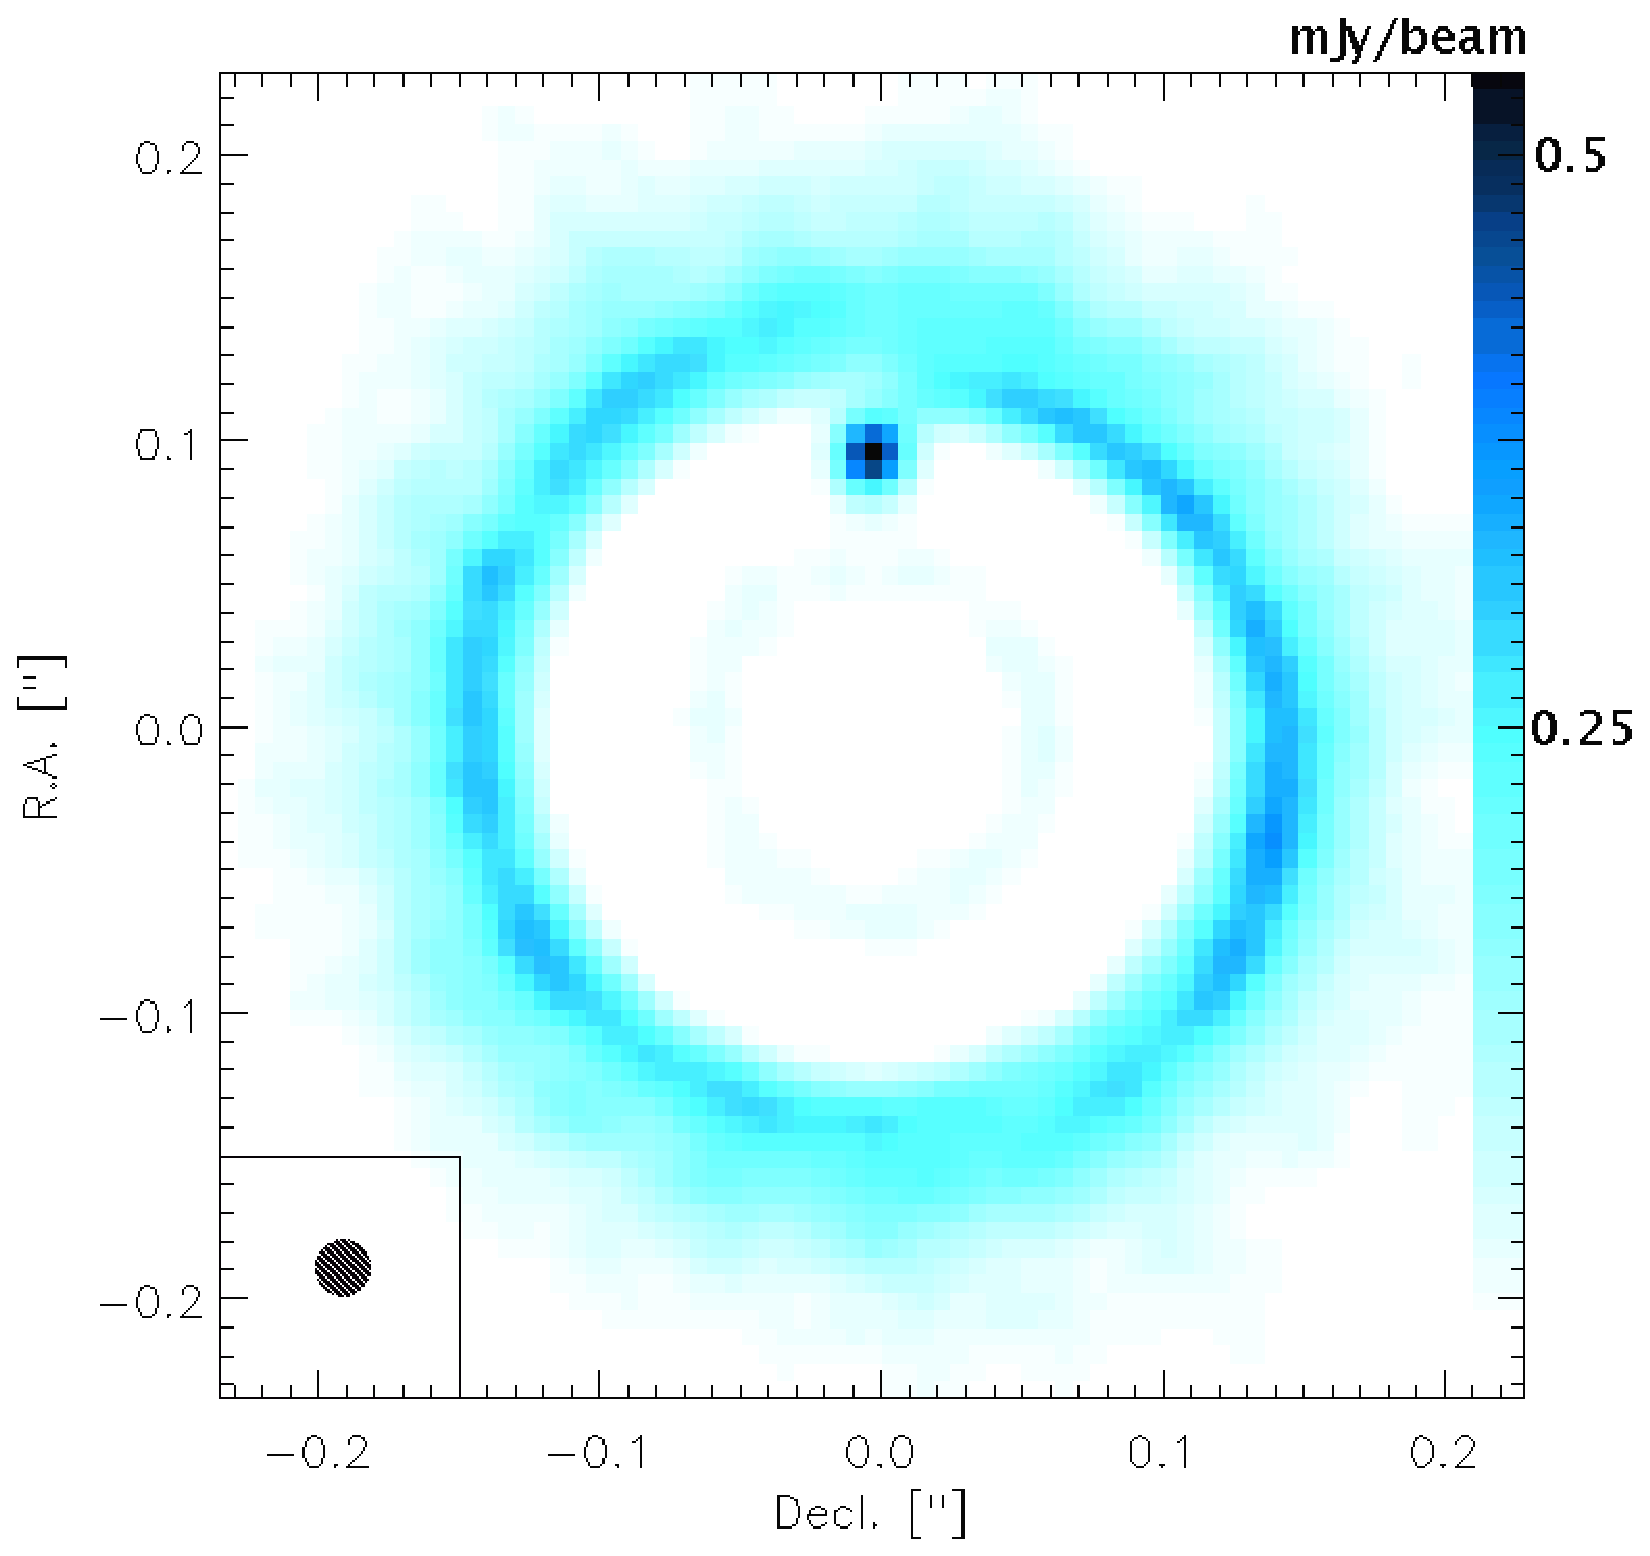
\includegraphics{d2fig1a.eps}}
    \hspace*{5mm}
%    \resizebox{0.45\hsize}{!}{\includegraphics{alma_100pc.eps}}
    \resizebox{0.45\hsize}{!}{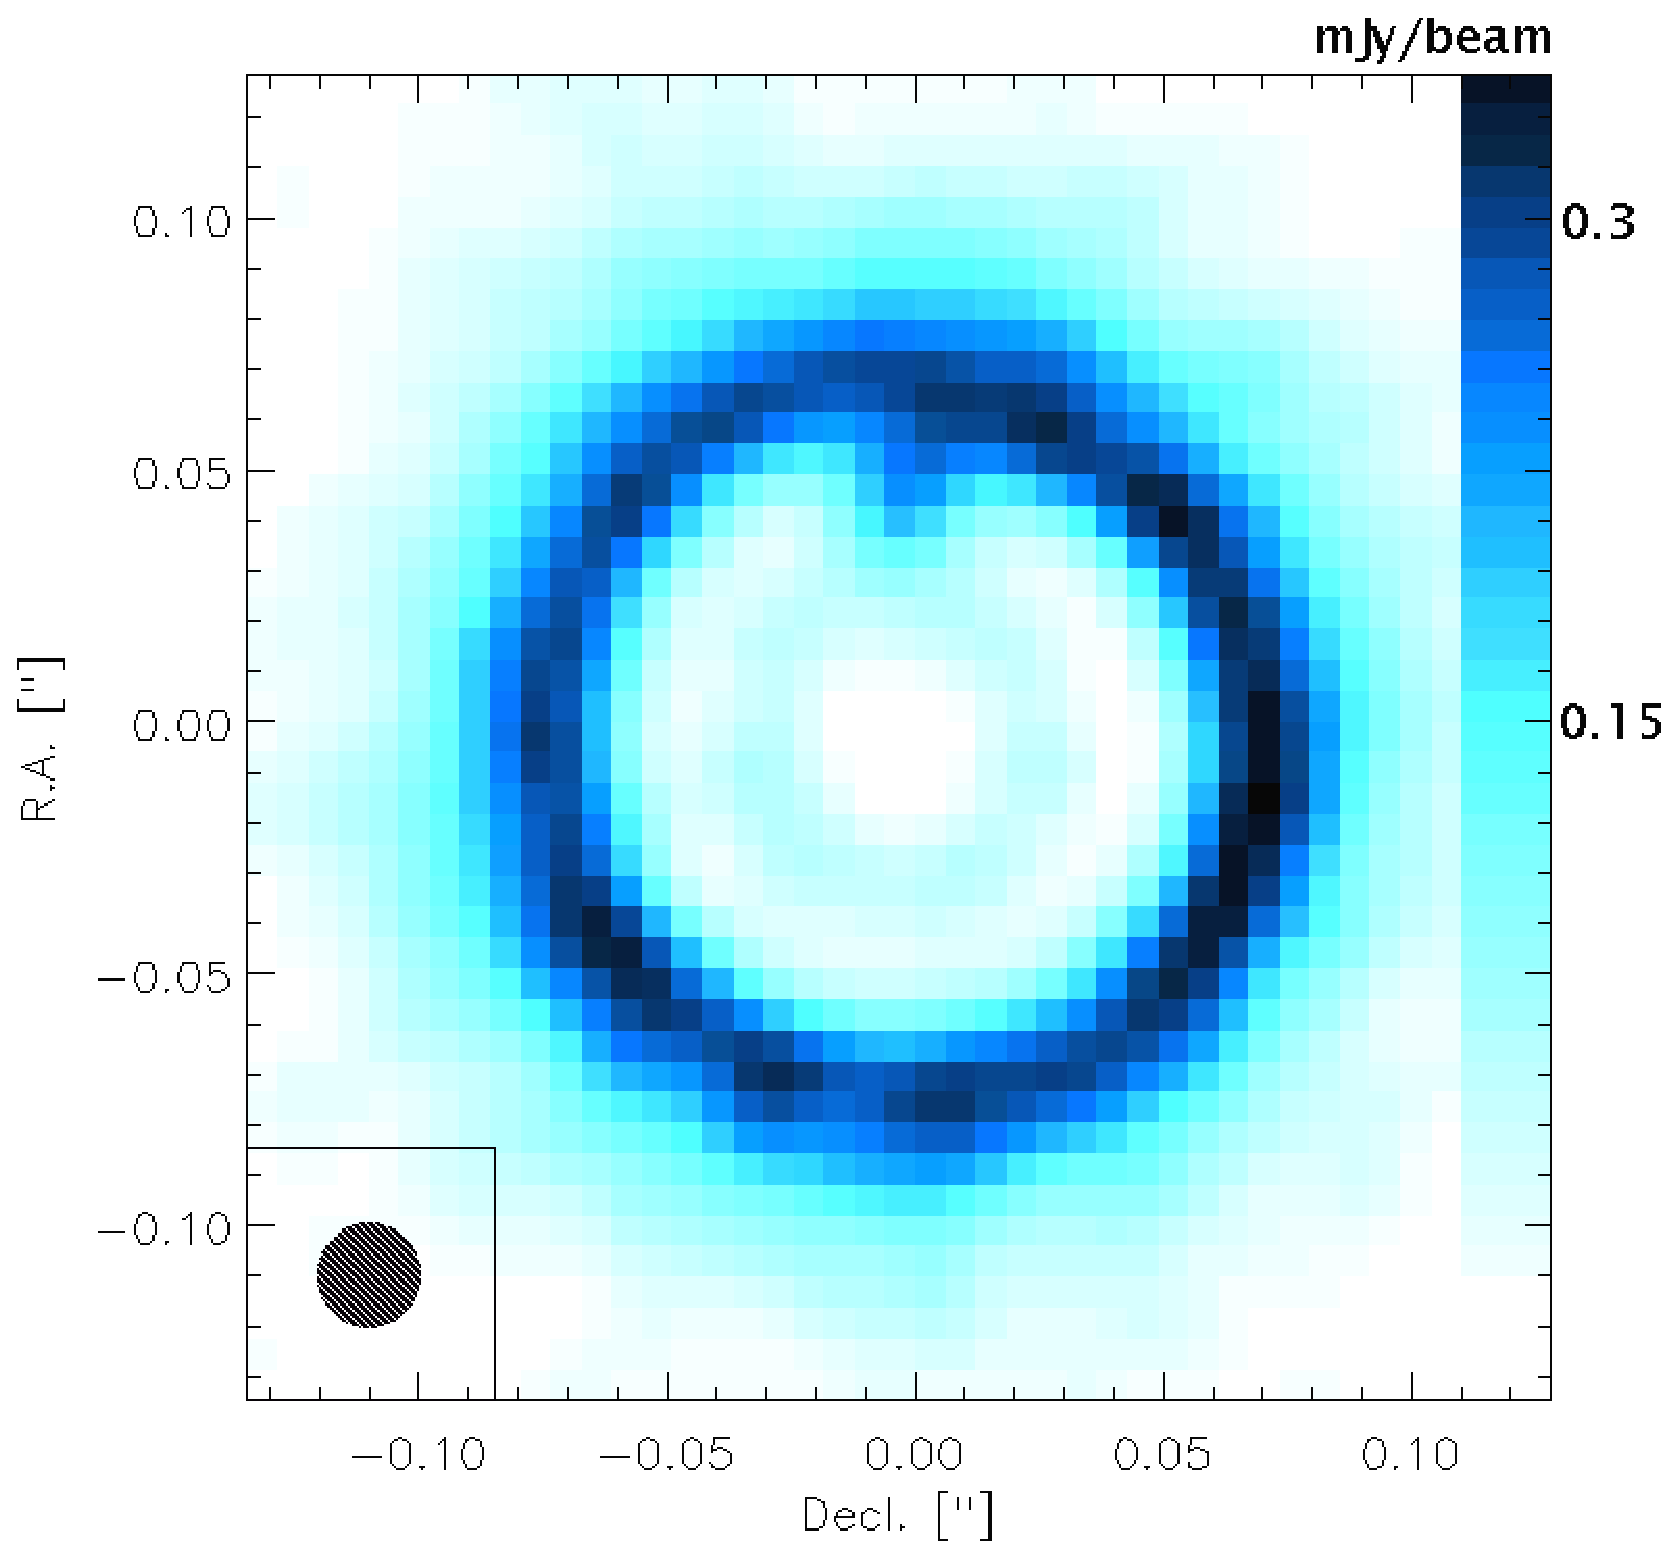
\includegraphics{d2fig1b.eps}}
  \end{center}
  \caption{Example for the application of the radiative transfer software {\tt MC3D}.
%    using hydrodynamic input data to make model predictions for telescopes, in this case {\em ALMA}.
    Here, a three-dimensional hydrodynamic model of a disk with an embedded planet with a mass of
    $1\,{\rm M_{\rm jup}}$ around a $0.5\,{\rm M_{\rm sun}}$ star (orbital
    radius: 5\,AU) has been used to investigate the feasibility
    to observe the planet and structures in the disk caused by the planet-disk interaction
    with {\em ALMA} (assumed distance is 50\,pc [left] / 100\,pc [right]).
%    The disk mass amounts to $M_{\rm disk} =
%    1.0\times10^{-2}\,{\rm M_{\rm sun}}$.  Only structures above the
%    $2\sigma$-level are shown.  
    The size of the combined beam is symbolized
    in the lower left edge of each image. Similar techniques will be
    used to derive observable quantities within the proposed project.
%    Note the reproduced shape of the
%    spiral wave near the planet and the slightly shadowed region behind the
%    planet in the left image.  
    {\em [from Wolf \& D'Angelo~2005]}
    \label{fig-giantplanet-alma}
    }
\end{figure}



%\noindent
%{\sl [a-2] Radiative transfer software in evolved, optically thin disks:} 
In addition to the {\tt MC3D} a radiative transfer tool was developed which
is optimized for the case of optically thin debris disks (Wolf \&
Hillenbrand~\cit{2005}).
%
% More specifically, it is optimized for studying arbitrarily structured,
% optically thin dust configurations where large grains (i.e., grains with a
% large size parameter) are expected to determine the far-infrared through
% millimeter dust reemission SED.  On the basis of optical properties of dust
% grains obtained through laboratory measurements, this software allows to
% derive scattered light and dust reemission SEDs for either analytically
% described dust density distributions or the direct implementation of the
% results of n-particle simulations.
%
This software has already been used in the context of theoretical studies
concerning the appearance of debris disks (Wolf \& Hillenbrand~\cit{2003};
Moro-Mart\'{\i}n, Wolf \& Malhotra~\cit{2005}) and for the analysis of
observed debris disk spectra (e.g., Sch\"utz et al.~\cit{2004}; Meyer et
al.~2004, Hollenbach et al.~2005; Kim et al.~2005;
Silverstone et al.~2006; Hines et al.~2006).

%We also have other radiative transfer tools available developed by the
%second PI. Of particular interest is a module for stochastic (quantum-)
%heating of very small grains and polycyclic aromatic hydrocarbons
%(Dullemond in prep.~{\bf XXXX}).
% This quantum module can, if necessary,
% also be built into {\tt MC3D}.


\subsection{Disk structure models}
%
Over the last years we developed various self-consistent models for the
structure of protoplanetary disks. Dullemond, Dominik \& Natta (\cit{2001})
presented a two-layer model similar to the model of Chiang \& Goldreich
(\cit{1997}), but with a treatment of the dust sublimation radius. They
argued that the dust inner rim (inward of which there is only gas, which is
presumably optically thin) is much hotter than the dusty disk behind it, and
is therefore presumably puffed-up. Moreover, we showed that the emission
from this inner rim can explain the near-infrared bump between 2 and 7
$\mu$m seen in nearly all Herbig Ae/Be star SEDs. We also developed more
detailed 1+1-D vertical structure models (Dullemond, van Zadelhoff \& Natta
\cit{2002}; Dullemond \& Natta \cit{2003a/b}), which are useful as a basis
on which calculations of the local physics can be done (e.g.~Kamp \&
Dullemond \cit{2005}). A final level of complexity was reached with models
based on 2D continuum radiative transfer (Dullemond \cit{2002}; Dullemond
\& Dominik \cit{2004a}). These models showed the possibility that the inner
regions of the disk might, under some circumstances shadow the outer disk regions
(in particular dust coagulation and sedimentation), causing these
to emit less strongly in the far-infrared. The discrepancy between the
flaring disks and the self-shadowed disks found in these models might
explain the different groups of SEDs observed for Herbig Ae stars (group I
and group II, Meeus et al.~\cit{2001}). 

We constructed models of dust sedimentation and coagulation which we
translated into observable features using a multi-dimensional radiative
transfer tool (Dullemond \& Dominik \cit{2004b}, \cit{2005}). The experience
gained in this work on coupling dust evolution models to radiative transfer
codes will be of direct use for the project proposed here.

Furthermore, we studied the effect of the disk formation and viscous evolution
history on the properties of disks observed at ages of typical T Tauri /
Herbig Ae stars. We have shown that the properties of the original core out
of which the star+disk system was formed may affect the level of
crystallinity of the dust in the disk (Dullemond, Apai \& Walch
\cit{2006}). We also show that such a simple model might explain the $\dot
M\propto M_{*}^2$ correlation observed in clusters (Dullemond, Natta \&
Testi \cit{ApJ, accepted}).

Depending on the goal we wish to address, these disk structure and 
evolution models will serve as a basis upon which radiative transfer
modeling will be performed in this project.

\subsection{Calculation of opacities and scattering properties of dust particles}
One of the crucial model parameters for the radiative transfer code outlined in Section~\ref{mc3d}
are the opacity and scattering properties (including the polarization of scattered radiation) 
of grains of various sizes and shapes. 
In this context, dust grains are in most applications considered to be spherical,
allowing to apply Mie theory.
In the particular case of circumstellar disks, broad grain size distributions
(grain radii $a$: nanometers -- millimeters)
and a very wide wavelength range ($\lambda \approx 10^{-10}-10^{-2}$\,m) of the interacting radiation have
to be considered. Previous numerical solutions to the Mie scattering problem are not appropriate to consider
size parameters $x=2\pi a/\lambda >10^4 - 10^5$.
In order to overcome this limitation, we developed a Mie scattering code which allows 
to calculate the optical properties of dust grains of arbitrary size (Wolf \& Voshchinnikov~2004).
Single scattering by particle ensembles is calculated by proper averaging of the respective parameters
(see also Wolf~2003b for a study of efficient radiative transfer in dust grain mixtures).
Furthermore, we have developed numerical algorithms for {\tt MC3D} which allow to consider
multiple light scattering in dust configurations containing aligned 
/ non-aligned non-spherical dust grains (Wolf et al.~2002b).


%spherical particles, Mie theory is often applied.  However, previous numerical
%solutions to the Mie scattering problem are not appropriate for particles
%that are very much larger than the wavelength of interest ($x=2\pi a/\lambda
%>10^4 - 10^5$). In disks with grain growth it is easy to get in this regime.
%In order to overcome this limitation, we developed a Mie scattering code
%which allows to calculate arbitrary size distributions / parameters (Wolf \&
%Voshchinnikov~\cit{2004}). Single scattering by particle ensembles is
%calculated by proper averaging of the respective parameters (see also
%Wolf~\cit{2003b} for a study of efficient radiative transfer in dust grain
%mixtures). 
%We have developed numerical algorithms for {\tt MC3D} (see [a-1]) which allow to consider
%multiple light scattering in dust configurations containing aligned 
%/ non-aligned non-spherical dust grains ().\\


% For reasons of simplicity dust grains are in most cases considered as
% homogeneous spheres in the modeling and interpretation of circumstellar
% disk observations.  However, in reality such particles and aggregates
% can have complex non-spherical structures
% 
% laboratory experiments of grain growth indicate
% that dust grains are expected to have a rather complex, possibly fractal
% structure 
% 
% (see Lumme \& Rahola~{\bf 1994} for porous dust particle light
% scattering).  Moreover, non-spherical grains are observed in star-forming
% regions through submillimeter polarimetry (e.g., Wolf, Launhardt \& Henning
% {\bf 2004}).  
% 
% In the optical to near-infrared wavelength range,
% non-centrosymmetric polarization patterns have been observed in bipolar and
% cometary nebulae (Scarrott et al.~1989), young stellar objects (Hajjar \&
% Bastien~1996), evolved stars (Kastner \& Weintraub~1996), and are also
% clearly seen in polarization maps of comets (Dollfus \& Suchail~1987).
% These findings as well as the wavelength dependence of the positional angle
% of polarization observed in red giants, AGB stars, and bipolar reflection
% nebulae (see, e.g., Johnson \& Jones~1991) and very high degrees of circular
% polarization of scattered light in the Orion molecular cloud, measured by
% Chrysostomou et al.~(2000), are considered to be caused by aligned
% non-spherical grains.  
% 
% \\
    


% ----------------------------------------------------------------------------------------
%\vspace*{5mm}
%\noindent
%{\bf [b] T Tauri Disk studies - Early Stages of Planet Formation}
%\vspace*{2mm}

%\noindent
\subsection{Deriving grain sizes from disk observations}\label{butter.model}
%{\sl [b-1] Dust grain evolution:}
We developed a radiative transfer model of the circumstellar environment of
the so-called ``Butterfly Star'' in Taurus (IRAS~04302+2247) - an edge-on
circumstellar disk (Wolf et al.~2003).  Our model is based on
multi-wavelength continuum observations: (1) Millimeter maps, and (2)
High-resolution near-infrared scattered light images obtained with {\em HST}/NICMOS.  The advantage
of the combination of both observations is that they trace (a) different
regions of the system and (b) different physical processes.  We find disk
and envelope parameters which are comparable with those of the circumstellar
environment of other young stellar objects. Most importantly, we find that the dust
properties must be different in the circumstellar disk and in the envelope.
While a grain size distribution with grain radii up to 100\,$\mu$m is
required to reproduce the millimeter observations of the disk, the envelope
is dominated by smaller grains similar to those of the interstellar medium.

Furthermore, we analysed the $\sim$\,10\,$\mu$m silicate
feature of 27 T\,Tauri stars.  Here, we assumed that this emission
feature can be represented by a linear superposition of the
wavelength-dependent opacity describing the optical properties of spherical
homogeneous silicate grains with different chemical composition, structure,
and grain size. We show that acceptable fitting
results can also be achieved if emission properties of porous silicate
grains are considered instead.  We conclude that -- in terms of the
pro\-perties of the circumstellar dust -- T\,Tauri systems are a
continuation of HAeBe systems at their lower mass end (Schegerer et
al.~2006). 


% {\sl [b-2] On the observability of giant planets in circumstellar disks:}
% We investigate the possibility to detect giant planets that are still embedded in young circumstellar disks
% (Wolf \& D'Angelo~2005, Wolf et al.~2003).
% Based on models with different stellar, planetary, and disk masses, and different radial positions
% of the planet we analyze the resulting submillimeter appearance of these systems. 
% We find that the influence of the planet on the SED could not be distinguished 
% from that of other disk parameters. However, dust reemission {\em images} of the disks show that the hot region 
% in the proximity of a young planet, along with the gap, could indeed be detected
% and mapped with the Atacama Large Millimeter Array in the case of nearby circumstellar disks (d$<$100\,pc)
% in approximate face-on orientation (see Fig.~\ref{fig1}).
% \\




%\noindent
%{\sl [c-1] Structures in Debris Disks:}
%A software has been developed to simulate the dynamical evolution of dust particles in debris disks
%under the influence of stellar gravity, planetary perturbations, radiation and stellar wind forces (Rodmann~2005).
%It allows to determine the equilibrium density structure of dust in debris disks.
%\\
%
%\begin{figure}[t!]
%  \begin{center}
%    \resizebox{0.34\hsize}{!}{\includegraphics{f16.eps}}
%   \hspace*{10mm}
%    \resizebox{0.50\hsize}{!}{\includegraphics{f7a.eps}}
%  \end{center}
%  \caption{
%{\em [Top left]} 
%Possible degeneracy between the grain chemical composition and the 
%location of the planet clearing the gap. $\it{Solid~line}$: SED of dust disk 
%composed of MgSiO$_3$ grains with a 3M$_{\rm Jup}$ planet at 1 AU; 
%$\it{dashed~line}$: same for MgFeSiO$_4$ grains with a
%3M$_{\rm Jup}$ planet at 30 AU.
%{\em [Middle/Bottom left]}
%Brightness density distributions at 70 $\mu$m (assuming graybody emission from 
%12 $\mu$m grains) expected from a disk with a 3M$_{\rm Jup}$ planet at 1\,AU (middle) and 30\,AU (bottom), 
%respectively.
%{\em [Right]}
%SEDs of disks composed of 40$\mu$m grains with different grain
%chemical compositions, for a model resembling the solar system
%(i.e., the planets, excluding Mercury and Pluto, and the Kuiper belt
%as the source of dust; top right) and the corresponding debris disk without planets (bottom right).
%{\sl [from Moro-Mart\'{\i}n, Wolf \& Malhotra~2005]}
%  }\label{ama_deg}
%\end{figure}
%\noindent
%{\sl [c-2] Spectroscopic Signatures of Debris Disks:}
%In anticipation of future observations 
%of spatially unresolved debris disks with the Spitzer Space Telescope, we studied
%how the structure carved by planets affects the shape of the disk's SED 
%and consequently whether the SED can be used to infer the presence of planets 
%(Wolf \& Hillenbrand 2003; Moro-Mart\'{\i}n, Wolf \& Malhotra~2005).
%We numerically calculate the equilibrium spatial density distributions and SEDs of dust disks originated 
%by a belt of planetesimals in the presence of interior giant planets in different planetary con gurations 
%and for a representative sample of chemical compositions. The dynamical models are necessary to estimate 
%the enhancement of particles near the mean motion resonances with the planets and to determine how many particles 
%drift inside the planet's orbit. On the basis of the SEDs and predicted Spitzer colors we discuss what types 
%of planetary systems can be distinguished and the main parameter degeneracies in the model SEDs (see Fig.~\ref{ama_deg}).
%\\


% ----------------------------------------------------------------------------------------
%\vspace*{5mm}
%\noindent
%{\bf [c] Simulating the evolution of solids in protoplanetary disks}
%\vspace*{2mm}

%\noindent

\subsection{Simulating the evolution of solids in protoplanetary disks}
A code was developed to track the evolution of solids in protoplanetary disks
from the early phase when they are in the form of small dust particles, till
the stage when most of them are locked in a planetesimal swarm or have been accreted
onto the central star. A number of simplifications and idealisations allows
to consider gas-particle coupling, coagulation, sedimentation, and
evaporation/condensation processes. At the same time the code remains
computationally efficient allowing to calculate large grids of models and to
investigate how different properties of the protoplanetary disk influence
the architecture of the nascent planetesimal swarm
% Using another developed
% code that describes giant planets formation by core accretion gas capture
% model, it allows us to identify the disk parameters which are key in
% determining the properties of Jupiter-like planets 
(see e.g., Kornet \& Wolf 2006; Kornet, Wolf \& R${\rm
\acute{o}\dot{z}}$yczka~2006). This code can be used optionally, i.e.,
complementarily to the input from projects C1 and C2.


%\begin{figure}
%\centerline{\includegraphics[width=8cm]{myfig.eps}}
%\caption{This is the figure caption text....}
%\end{figure}

%
% Here follows the own refereed publications by the PIs in relation to
% the project proposed here.
%

\newpage
%\vspace*{2mm}
\ownpubltitle{Own publications related to the Forschergruppe:}
%
% BELOW IS ONLY AN EXAMPLE OF TWO ENTRIES. SEE THE ADDITIONAL FILES 
% SENT TO YOU WITH ALL THE REFERENCES FROM THE VORANTRAG
%
\begin{ownpubl}
\item Agol, E., Barth, A., Wolf, S. and Charbonneau, D. (2003)
  Spectropolarimetry and Modeling of the Eclipsing T Tauri Star KH15D, 
  \apj, {\bf 600}, 781

\item Carpenter, J., Wolf, S., Schreyer, K., Launhardt, R. and Henning,
  Th. (2005) Evolution of Cold Circumstellar Dust Around Solar-Type Stars,
  \apj, {\bf 129}, 1049

\item {Dullemond}, C.~P. and {Apai}, D. and {Walch}, S. (2006)
  Crystalline Silicates as a Probe of Disk Formation History, 
  \apjl, \textbf{640}, 67

\item {Dullemond}, C.~P. and {Dominik}, C. (2005) Dust coagulation in
  protoplanetary disks: A rapid depletion of small grains, 
  \aap, \textbf{434}, 971

\item {Dullemond}, C.~P. and {Dominik}, C. (2004b) The effect of dust
  settling on the appearance of protoplanetary disks, \aap
  \textbf{421}, 1075 

\item {Dullemond}, C.~P. and {Dominik}, C. (2004a) Flaring
  vs. self-shadowed disks: The SEDs of Herbig Ae/Be stars, \aap,
  \textbf{417}, 159

\item {Dullemond}, C.~P. and {Natta}, A. (2003b) An analysis of two-layer
  models for circumstellar disks, \aap, \textbf{405}, 597

\item {Dullemond}, C.~P. and {Natta}, A. (2003a) The effect of scattering on
  the structure and SED of protoplanetary disks, \aap, \textbf{408}, 161

\item {Dullemond}, C.~P. and {van Zadelhoff}, G.~J. and {Natta}, A.
  (2002) Vertical structure models of T Tauri and Herbig Ae/Be disks,
  \aap, \textbf{389}, 464 

\item {Dullemond}, C.~P. (2002) The 2-D structure of dusty disks around
  Herbig Ae/Be stars. I.  Models with grey opacities, \aap, \textbf{395}, 853

\item {Dullemond}, C.~P., {Dominik}, C. and {Natta}, A. (2001)
  Passive Irradiated Circumstellar Disks with an Inner Hole, \apj,
  \textbf{560}, 957

\item {Dullemond}, C.\ P. and {Turolla}, R. (2000) An efficient algorithm
  for two-dimensional radiative transfer in axisymmetric circumstellar
  envelopes and disks, \aap, \textbf{360}, 1187

\item Eisner, J.A., Hillenbrand, L.A., Carpenter, J.M. and Wolf, S. (2005)
  Constraining the Evolutionary Stage of Class I Protostars:
  Multi-Wavelength Observations and Modeling, \apj, {\bf 635}, 396

\item Hines, D.C., Backman, D.E., Bouwman, J., Hillenbrand, L.A., Carpenter,
  J.M., Meyer, M.R. et al.
%  Kim, J.S., Silverstone, M.D., Rodmann, J., Wolf, S.,
%  Mamajek, E.E., Brooke, T.Y., Padgett, D.L., Henning, Th., Moro-Martin, A.,
%  Stobie, E., Gordon, K.D., Misselt, K., Morrison, J., Muzerolle, J., Su,
%  K. 
  (2006) The Formation and Evolution of Planetary Systems (FEPS):
  Discovery of an Unusual Debris System Associated with HD 12039, \apj, in
  press

\item Hollenbach, D., Gorti, U., Meyer, M., Kim J.S., Morris, P., Najita,
  J., Pascucci, I., Carpenter, J., Rodmann, J., Brooke, T., Mamajek, E.,
  Padgett, D., Soderblom, D., Wolf, S. and Lunine, J. (2005) Formation and
  Evolution of Planetary Systems: Upper Limits to the Gas Mass in HD 105,
  \apj, 631, 1180

\item {Kamp}, I. and {Dullemond}, C.~P. (2004) The Gas Temperature in the
  Surface Layers of Protoplanetary Disks, \apj, \textbf{615}, 991 

\item Kim, J.S., Hines, D.C., Backman, D.E., Rodmann, J., Hillenbrand, L.A.,
  Moro-Martin, A., Carpenter, J.M., Silverstone, M.D., Bouwman, J., Mamajek,
  E.E., et al.
%  Meyer, M.R., Wolf, S., Malhotra, R., Pascucci, I., Najita, J.,
%  Henning, Th., Brooke, T.Y., Strom, S.E., Padgett, D.L., Stobie, E.B.,
%  Engelbracht, Ch., Gordon, K., Misselt, K., Morrison, J., Muzerolle, J.,
%  Su, K.Y.L. 
  (2005) Formation and Evolution of Planetary Systems: Cold Outer
  Disks Associated with Sun-like stars, \apj, 632, 659

\item Kornet, K. and Wolf, S. (2006)
  Radial distribution of planets. Predictions based on the Core Accretion / Gas Capture model for planet formation,
  \aap, in press

\item Kornet, K., Wolf, S. and R${\rm \acute{o}\dot{z}}$yczka, M. (2006)
  Planet formation around stars with various masses,
  \aap, in press

\item Meyer, M.R., Hillenbrand, L.A., Backman, D.E., Beckwith, S.V.W., Bouwman, J., Brooke, T.,Y., 
  Carpenter, J.M., Cohen, M., Gorti, U., Henning, Th., et al. (2004)
  \titl{The Formation and Evolution of Planetary Systems: First Results from a Spitzer Legacy Science Program},
  \apjs, 154, 422

\item Metchev, S.A., Eisner, J.A., Hillenbrand, L. and Wolf, S. (2005) 
  Adaptive Optics Imaging of the AU Microscopium Circumstellar Disk -- Evidence for Dynamical Evolution,
  \apj, {\bf 622}, 451

\item Moro-Mart\'{\i}n, A., Wolf, S. and Malhotra, R. (2005)
  Signatures of Planets in Spatially Unresolved Debris Disks,
  \apj, 621, 1079

\item Pascucci, I., Henning, Th., Steinacker, J. and Wolf, S. (2003)
  2D/3D Radiative Transfer Codes to Analyze and Predict VLTI observations,
  \textit{Astroph. \& Space Science}, {\bf 286}, 113

\item Pascucci, I., Wolf, S., Steinacker, J., Dullemond, C.P., Henning, Th., Niccolini, G., Woitke, P.
  and Lopez, B. (2004)
  The 2D Radiative Transfer Problem - Benchmark Results for Disk Configurations, 
  \aap, {\bf 417}, 793

%\item Rodmann, J. (2006) PhD thesis, University Heidelberg

\item Schegerer, A., Wolf, S., Voshchinnikov, N.V., Przygodda, F. and Kessler-Silacci, J.E. (2006)
  Analysis of the dust evolution in the circumstellar disks of T Tauri stars, 
  \aap, in press

\item Sch\"utz, O., Nielbock, M., Wolf, S., Henning, Th. and Els, S. (2004)
  SIMBA's view of the epsEri disk, 
  \aap, {\bf 414}, L9

\item Silverstone, M.D., Meyer, M.R., Mamajek, E.E., Hines, D.C., Pascucci, I., Hillenbrand, L.A., Bouwman, J., 
  Kim, J.M. et al.
%  Carpenter J.M., Stauffer, J.R., Najita, J., Moro-Martin, A., Henning, Th., Wolf, S., Backman, D.E., 
%   Brooke, T.Y., Padgett, D.L. 
  (2006)
  Formation and Evolution of Planetary Systems (FEPS): Primordial warm dust evolution from 3-30 Myr around Sun-like stars
  \apj, in press

\item Wolf, S. (2001a) 
  Dreidimensionaler Kontinuumsstrahlungstransport basierend auf der Monte-Carlo-Methode. Grundlagen und Anwendungen, 
  PhD thesis, Friedrich Schiller University Jena (Germany)

\item Wolf, S., (2001b)
  Inverse raytracing based on the Monte-Carlo method, 
  \aap, {\bf 379}, 690

\item Wolf, S. (2003a)
  MC3D - 3D Continuum Radiative Transfer, Version 2
  \textit{Computer Physics Communications}, {\bf 150}, 99

\item Wolf, S. (2003b)
  Efficient radiative transfer in dust grain mixtures, 
  \apj, {\bf 582}, 859

\item Wolf, S. and D'Angelo, G. (2005)
  On the Observability of Giant Protoplanets in Circumstellar Disks, 
  \apj, {\bf 619}, 1114

\item Wolf, S., Fischer, O. and Pfau, W. (1998) 
  Radiative transfer in the clumpy environment of young stellar objects, 
  \aap, {\bf 340}, 103

\item Wolf, S., Gueth, F., Henning, Th. and Kley, W. (2002a)
  Detecting planets in protoplanetary disks: A prospective study, 
  \apj, {\bf 566}, L97

\item Wolf, S. and Henning, Th. (2000)
  Accelerated self-consistent radiative transfer based on the Monte-Carlo method, 
  \textit{Computer Physics Communications}, {\bf 132}, 166

\item Wolf, S., Henning, Th. and Stecklum, B. (1999)
  Multidimensional self-consistent radiative transfer simulations based on the Monte-Carlo method, 
  \aap, {\bf 349}, 839

\item Wolf, S. and Hillenbrand, L. (2003)
  Model Spectral Energy Distributions of Circumstellar Debris Disks. 
  I. Analytic Disk Density Distributions, 
  \apj, {\bf 596}, 603

\item Wolf, S. and Hillenbrand, L. (2005)
  Debris disk radiative transfer simulator,
  \textit{Computer Physics Communications}, {\bf 171}, 208

\item Wolf, S. and Klahr, H. (2002)
  Large-scale Vortices in Protoplanetary Disks: 
  On the observability of possible early stages of planet formation, 
  \apj, {\bf 578}, L79

\item Wolf, S., Moro-Mart\'{\i}n, A. and D'Angelo, G. (2006)
  Signatures of Planets in Protoplanetary and Debris Disks, 
  \pss, submitted

\item Wolf, S., Padgett, D.L. and Stapelfeldt, K.R. (2003)
  The Circumstellar Disk of the Butterfly Star in Taurus, 
  \apj, {\bf 588}, 373

\item Wolf, S. and Voshchinnikov, N.V. (2004)
  Light scattering by very large grains, 
  \textit{Computer Physics Communications}, {\bf 162}, 113

\item Wolf, S., Voshchinnikov, N.V. and Henning, Th. (2002b)
  Multiple scattering of polarized radiation by non-spherical grains: first results, 
  \aap, {\bf 385}, 365

\end{ownpubl}
%

%\newpage
\section{Goals (Ziele)}\label{goals}

The general goal of this project is to provide a link between the results of
the laboratory and numerical experiments of this Forschergruppe and
astronomical observations of planetesimal-forming/harbouring circumstellar
disks. In particular, the direct comparison of observable quantities
with existing or future observations will allow to verify the models for the different
phases of planetesimal formation derived by the other teams of the Forschergruppe.

Moreover, the goal is to identify the (combinations of) observable quantities which allow to trace the evolution
of the dust / disk in the potentially planetesimal-forming region 
(based on the simulation of the SED, spatially resolved, wavelength-dependent polarization and intensity maps 
in scattered and/or reemitted radiation, and interferometrically observable quantities).
Based on the input from the projects A1, A2, B2, C1, C2, and D1, questions to be addressed,
mainly through parameter space studies, are\footnote{If certain questions rely on the input
from selected projects only, these projects are indicated in brackets. Otherwise, all projects apply.}

\begin{enumerate}

\item Is it possible to constrain the radial mixing efficiency traced by crystalline grains? [A1,A2]
  
\item To which extent can the vertical disk structure (as a function of the radial distance from the central star), 
  and thus the processes of dust settling, vertical mixing, and growth be constrained observationally? [A1,B2,C2]

\item Which complementary constraints about the size and structure 
  of dust grains can be derived from polarization measurements? [A1,B2,C2]
  
\item How do the observable quantities change during the early evolution of protoplanetary disks?
  (Rem.: The evolution will at first be parameterized by a decrease of the mass of submicron-sized dust grains.
  As a second step, the numerical description of the grain size distribution from project [\projdul{}]
  will be taken into account.)
  
\item What is the potential of combining spectrally resolved high spatial resolution imaging (milliarcsecond scale) 
  obtained in the mid-infrared wavelength range accessible from the ground (L,M,N,Q band) to significantly better
  constrain the chemical composition and size of dust grains than using the prominent $\sim$10\,$\mu$m 
  silicate feature alone? [A1,A2,B2,C2]
    
\item To which extent can the concentration of millimeter to centimeter-sized grains
  in anticyclonic vortices, spiral waves, and in/around turbulent eddies
  in the outer regions of protoplanetary disks be traced? [C1,B2]
  
\item Are short-term temporal variations on the timescale of years or less of any of the observable quantities expected 
  (particularly of those tracing the inner $<$\,1\,AU\,\ldots\,few AU planet forming regions of protoplanetary disks)?

\item Which infrared spectral signatures of protostars can be inferred from the early solar system mineralogy? [D1]

\item Which observations are needed to constrain the location of the snow-line traced by ices?
  
\item Which are the minimum / optimum requirements for the proposed observations, in terms of, e.g.,
  spatial resolution, wavelength range/coverage, spectral resolution, sensitivity, and accuracy?
  
\item What is the sensitivity / accuracy required to investigate the chemical composition of the smallest fragments
  resulting from planetesimal collisions in debris disks - as tracers for the chemical composition of planetesimals
  (taking into account the extremly low / undetected mid-infrared excess observed in the case of a significant fraction
  of debris disks with the Spitzer Space Telescope so far)?
  Which are the requirements for future space missions (using high-resolution imaging / nulling interferometry)? [A1,B2,D1]
  
\item What is the potential of combining near- to mid-infrared spectra obtained from space missions,
  tracing the global disk appearance,
  with spatially resolved interferometric observations of the planet forming region, obtained from the ground,
  but with a much more restricted wavelength-coverage?
  
\item What is the potential of spectro-interferometric observations with the VLTI in terms of constraining
  the dust evolution, using the current and planned 2$^{\rm nd}$ generation instrumentation in different wavelength regions
  (tracing scattered vs.\ reemitted radiation)? The results of this study will have direct impact on the
  science case studies for the 2$^{\rm nd}$ generation interferometric instruments MATISSE and VSI
  (Remark: The PI of this project is Project Scientist/Co-PI of MATISSE and Member 
  of the science team of the VLTI Spectro-Imager [VSI]).
\end{enumerate}

In order to address these questions (and those resulting from these studies),
a flexible radiative transfer modeling setup will be developed, based on the profound
preliminary work outlined in Section~\ref{prelim}.
The basis for this will be a disk model, implemented in the radiative transfer simulation tool {\tt MC3D}, 
with following specifications:
\begin{itemize}  
\item The model shall allow a detailed analysis of the dependence of observable quantities on
  the radial and vertical distribution of 
  a) the size distribution and
  b) the chemical composition and structure of dust grains.
  In particular, porous grains (important for the earliest stage of growth), 
  ice-mantled grains, and PAHs have to be considered.
\item Self-consistent solution of the vertical disk structure and the sublimation region of dust grains / ice mantles on grains
  (depending on the radial and vertical location in the disk).
%\item For the extension of the investigation towards more evolved disks, the effects of
%  radiation pressure, Poynting-Robertson effect, and the effect of photophoresis are to be considered in a self-consistent manner.
\item Similar to previous studies (see Section~\ref{mc3d}) software interfaces have to be developed which allow
  to implement 
  a) the optical properties derived in project A1 and
  b) the density and grain size distributions from projects A2, B2, C1, C2, and D1.
\end{itemize}

%A flexible radiative transfer modeling setup will be developed that
%will allow us to test the observational effect of various results from the Forschergruppe.
%Conversely, with this setup we will explore which aspects of
%the growth process from dust to planetesimals might be responsible for
%certain well-known observational facts of protoplanetary disks such as the
%existence of large inner holes, the existence and radial abundance
%variations of crystalline silicates, the observed grain sizes etc. .

%The particular goals to be targeted are the following:
%\begin{enumerate}
%\item \label{goal-c2} Constrains on grain size distributions and grain growth
%  in young gas-rich disks, in close collaboration with C2, with additional
%  input from projects C1, B2 and B4. From the model toward the observations,
%  we intend to:
%  \begin{enumerate}
%  \item Put constraints on processes of dust settling, vertical mixing
%    and growth from direct and indirect observations of the disk
%    geometry and vertical structure. For this we will use both infrared
%    spectral energy distributions as well as imaging.
%  \item Set limits on radial drift of dust by comparing models with
%    different radial drift efficiencies to observations.
%  \item Identify ways in which the study of observable dust grains
%   ($a\lesssim 1$ mm) in protoplanetary disks by infrared and
%   (sub-)millimeter telescopes provide clues to the {\em unobservable}
%   process of growth from $a\sim 1$ mm to multi-kilometer
%    planetesimals.\label{dulgoal-linkobs}
%  \item Identify ways in which the observable grains in the {\em surface
%    layers} of the disk provide clues to the unobservable grains {\em
%    deeply embedded within the disk}.
%  \end{enumerate}
%  Conversely, there are well-known recent observational peculiarities of
%  disks observed, which we intend to address by putting them in the 
%  context of the models:
%  In addition to this we will attempt to solve some of the observational
%  mysteries listed above using the combination of the coagulation and
%  radiative transfer models.
%  Of these above observational aspects we will fully address only those for
%  which we, in the course of the Forschergruppe, find possible explanations
%  in terms of the research of this Forschergruppe and/or earlier known
%  physics.
%\item \label{goal-d1} A mineralogical comparison between the solar system
%  and protoplanetary disks, in close collaboration with project D1:
%  \begin{enumerate}
%    \item Comparison of mineralogical composition of Calcium-Aluminium-rich
%      Inclusions (CAIs, i.e.~the oldest components of meteorites originating
%      from undifferentiated planetesimals) with the mineralogy of
%      protoplanetary disks as derived from infrared spectroscopy.
%    \item Search for water-alterated minerals (phyllosilicates) in 
%      protoplanetary disk infrared spectra, as a hint for the presence of
%      large planetesimals in young gas-rich disks. 
%    \item {\bf MARIO: Are there other ways by which one could check
%      for planetesimals? Perhaps check for typical minerals in 
%      differentiated planetesimals? Basalts? What would such minerals
%      look like?}
%    \item In general: search for new minerals in the infrared spectra
%      of protoplanetary disks, based on minerals found in meteorites.
%  \end{enumerate}
%\item \label{goal-a2} Constraints on radial mixing of minerals from infrared
%  observations of protoplanetary disks, in close collaboration with project
%  A2. Insert model predictions of mineral abundances as a function of radius
%  from project A2 into the radiative transfer model to predict:
%  \begin{enumerate}
%    \item infrared spectra of the full disk and compare to e.g.~Spitzer
%    Space Telescope spectra.
%    \item infrared spectra {\em as a function of radius} and compare with
%      data from the VLT-MIDI interferometer and the VLT-VISIR camera.
%  \end{enumerate}
%  Derive constraints on the solid-state chemistry in disks and on the radial
%  mixing efficiency of the turbulence in the disk (the Prandtl number).
%\item Constrains on the location of intermediate-size bodies in 
%  gas-poor final stages of disks (debris disks).
%\item Investigate instrumental requirements, observational conditions and
%  feasibility of the above mentioned observations. Identify (and study the
%  feasibility of) potential new ways in which current/future observational
%  techniques (and combinations thereof) can be linked to the results from
%  the Forschergruppe. For instance:
%  \begin{enumerate}
%  \item Mineralogical analysis of {\em debris disks} using infrared
%    spectroscopy. Since this dust arises from planetesimal collisions {\em
%    only}, this allows us to `get a look inside' of planetesimals around
%    other stars.  Is such a study feasible in the light of the very weak
%    infrared excess of debris disks? If so, do they consist of similar
%    materials as the meteorites from our own solar system?
%  \end{enumerate}
%\end{enumerate}



\section{Work schedule (Arbeitsprogramm)}

\subsection{Methods}\label{methods}
The key task of this project is to derive observational constraints for the
evolution of solids in circumstellar disks. Both the initial conditions
(submicron-sized dust grains) and early evolution of these solids (growth
via coagulation to $\sim$\,mm-sized particles) can be observed directly in
the optical to millimeter wavelength range. Bodies larger than $\sim$1\,cm
cannot be traced directly.  However, these bodies of centimeter to
planetesimal size strongly influence the small grain population -- a
population which dominates the appearance of disks through their entire
evolution.  This is because collisions of larger bodies create fragments
which allow to trace the location, abundance, and chemical composition of
the cm to $\sim$ few km sized parent bodies. 
Possibilities to probe these larger bodies
indirectly will be investigated by combining detailed models of the growth and fragmentation processes 
-- studied in the various Forschergruppe projects -- with detailed radiative transfer tools. 
Very large bodies (planets) also affect the dust population by their
gravity. This can be very important for the structure and thus the appearance of disks,
but we will account for this only if it is essential for particular questions
because the Forschergruppe is focused on bodies up to a few hundred kilometers in size only.

We will consider various kinds of observations to trace the size distribution of the particles in the disk
as well as the mineralogical composition. As outlined before, the main analysis tool will be a radiative 
transfer tool set which allows the easy insertion of results from the Forschergruppe as input
physics, and therefore allows a direct link between experiments and models 
on the one hand and observations on the other hand.

%Since we wish to address many different issues (linking as much as possible
%the Forschergruppe to observations), it will be essential to consider a
%broad range of telescopes and instruments for which there is already a
%large volume of archival data and/or for which we have collaborations with
%teams which have access to such data. Here is a list of telescopes and 
%instruments which are useful/important for our project, and why:
%\begin{itemize}
%\item[{\em Spitzer-IRS:}] The Infrared Spectrograph on board the Spitzer
%Space Telescope yields the most sensitive infrared spectroscopy to date, in
%the range of 5 - 38 $\mu$m. Archival data exists for Herbig Ae/Be stars
%({\bf XXXXX}), T Tauri stars (e.g.~Kessler-Silacci et al.~\cit{2006}) and
%even a number of Brown Dwarfs (Apai et al.~\cit{2006}). This wavelength
%ranges covers the 10 $\mu$m Si-O resonance feature of silicates, including
%the peaks of various crystalline silicates such as forsterite, enstatite,
%all of which have been identified in such spectra already. The range between
%20 and 38 $\mu$m contains various bands of forsterite at lower temperatures,
%probing the somewhat more outer regions of the disk, where the presence of
%such crystals is closely linked to theories of radial mixing (project A2).
%The entire spectral range also covers potential peaks of the various
%minerals identified in meteorites (see Fig.~{\bf XXXXXXX}). The second PI
%is member of the Spitzer Legacy Team ``cores to disks'', and therefore has
%access to high-quality reduced data for hundreds of protoplanetary disks.
%\item[{\em VLT-MIDI:}] The MIDI instrument on the Very Large Telescope is a
%mid-infrared interferometer, allowing to obtain 8-13 $\mu$m spectroscopy
%{\em as a function of distance from the star}, basically resolving from
%$\sim$1 AU out to $\sim$20 AU for disks at typical distances to Earth. Since
%the 10 $\mu$m feature shape tells about the size and composition of the
%dust, this can be directly linked to theories of radial mixing, as well as
%theories of grain growth, sedimentation and vertical mixing. MIDI has been
%built at the Max-Planck-Institute for Astronomy, there is excellent access
%to high-quality data. A follow-up of MIDI, called MATISSE, is in planning.
%The first PI of this proposal is Project Scientist/Co-PI of MATISSE and
%Member of the science team of the VLTI Spectro-Imager [VSI].
%\item[{\em VLT-VISIR:}] VISIR on the Very Large Telescope is a spectrograph and
%imager in the N and Q-band (8-13 $\mu$m and 16.5-24.5 $\mu$m), with the
%diffraction-limited spatial resolution of the 8-meter single VLT
%telescope. For disks at typical distances one can resolve down to 
%about 20 AU distance from the central star, complementing the resolving
%power of VLT-MIDI.
%\item[{\em Optical imaging:}] {\bf Sebastian: polarimetry?? here I have very
%little knowledge} {\bf LINC-NIRVANA?}
%\item[{\em Millimeter observations:}] With various telescopes (Plateau de
%Bure; Very Large Array) a number of authors have obtained (sub-)millimeter
%maps of the outer regions of disks ($\gtrsim$ 50 AU) looking for evidence of
%large ($\gtrsim$ 1 mm) grains in these regions ({\bf XXXX}). It is the only
%current method of obtaining direct evidence for grains in the mm and cm size
%regime (direct evidence for larger grains is impossible), albeit only in the
%outer disk regions. Data available in the literature.
%\item[{\em Future: SOFIA, HERSCHEL:}] The SOFIA telescope on board a
%Boeing 747 is expected to fly within the next few years. The
%SAFIRE-spectrograph covers 145 - 655 $\mu$m, which is important for 
%obtaining the SEDs of disks (i.e.~hints on the disk geometry). In the
%somewhat more distant future the
%HERSCHEL Space Telescope will fly with the PACS instrument on board
%(in which MPIA has a part in the development), which covers 57-210 $\mu$m.
%This wavelength range includes many features of minerals contained in
%meteorites (see figure {\bf XXXX}) {\bf MARIO: PLEASE CHECK!}, and we
%can make predictions for this instrument.
%\item[{\em Future: ALMA:}] The Atacama Large Millimeter Array will, when
%on-line, be able to probe the distribution of grains with sizes up to
%millimeters throughout the disk. The spatial resolving power will allow
%to detect clumpiness or the concentration of grains in spiral waves. These
%are both features that are predicted by theory, in particular in project
%C1. In collaboration with C1 we can therefore predict what kind of
%patterns ALMA might find.
%\end{itemize}

\vspace{1em}
\noindent{\bf\em Modeling tools:}\\
\noindent 
In the framework of the proposed project various numerical methods will have
to be applied (see Section~\ref{prelim} for a more detailed description):

\begin{enumerate}
\item {\em Continuum radiative transfer calculations}\\
%
To derive observable quantities from the results of the Forschergruppe a
multi-dimensional radiative transfer code is required. The PIs of this
project have profound experience in the field of the development and
applications of radiative transfer codes, in particular in the field of
circumstellar disks. Although the PhD student will primarily apply existing
radiative transfer tools, necessary improvements of these are part of the
project as well. 

We will use the three-dimensional continuum radiative transfer code {\tt
MC3D} to compute spectra, wavelength-dependent intensity and polarization
maps, and derived quantities (such as interferometric visibilities).  This
software is highly flexible, allowing to adapt all relevant parameters of
the dust/disk model, such as the dust density distribution in the disk, the
optical properties of an arbitrary number of dust species, the grain
size distribution, etc.\,.  It is well-tested and has been applied for
similar purposes earlier (see Section~\ref{prelim}).

%Additions to the code, to be developed within this project:
%\begin{itemize}
%\item 
For modeling disks with very small grains, stochastic (quantum-)
heating has to be taken into account. The second PI has a module for
quantum-heated grains in his radiative transfer code {\tt RADMC}.  Since for
practical reasons we intend to use a single code in this project, rather
than switching between codes, we plan to implement this module into the
{\tt MC3D} code.
%\item To enable quick interactive modeling, we intend to parallelize the
%code using a very simple trick: instead of one run with, say, $10^7$ photons
%we will do 100 runs with $10^5$ photons, and average the resulting
%temperature profiles in a suitable way. This cheap method of
%parallelization, which requires no extra changes to the program, will be
%implemented and tested.
%\end{itemize}

\item {\em Codes for computing the opacity and scattering properties of
grains/aggregates}\\
%
Since we wish to study disks in which grain growth has possibly proceeded to
very large sizes, we will calculate the opacities and scattering properties
of the grains using a special Mie code developed by Wolf \& Voshchinnikov~(2004).
This code is able to treat grains with sizes well beyond $10^4$ times
the wavelength of interest. For treating grains with ice mantels and/or
porous structure we will use codes which are available to the team through
collaboration with N.V.~Voshchinnikov. 

Certain aggregation mechanisms, however, tend to yield very `fluffy'
(fractal) aggregates (e.g.\ Kempf et al.~1999). 
%The opacity of such
%aggregates is notoriously difficult to calculate. 
Min et al.~(2006) computed opacities of fractal grains using the Discrete Dipole
Approximation, and have shown that the opacity of large fractal grains with
low fractal dimension still looks like that of their much smaller
constituent particles. They propose an equivalent homogeneous and equivalent
porous grain who's opacity (at least in the 10 $\mu$m feature) is equivalent
to that of the bigger fractal grain. This is one of the possible ways 
in which the fractal structure of aggregates can be included in the models.

\item {\em Disk density structure and evolution models}\\
%
A radiative transfer tool can only predict spectra and images for a disk of
which the density structure is known beforehand. We have multiple years of
experience in self-consistent disk structure- and evolution model
development (see Section~\ref{prelim}). This experience, and the available
1+1D and 2D disk structure model tool sets, will provide the basis of the
models of this project. In principle, projects A2 and C1 will also yield
full-fledged disk structure models which can serve as the basis of the
radiative transfer calculations, but for flexibility we will also have our
own models available.
\end{enumerate}

\vspace{1em}
\noindent{\bf\em Observations:}\\
\noindent Considering the wide field of the intended comparisons of the
Forschergruppe results to observations we will, for a large part, rely on
archival data.  In addition, we will outline future observation strategies
to be followed for addressing particular issues.
However, in particular in the advanced stages of
the project (year 2 and 3), we keep the possibility open of writing
dedicated observing proposals and
analyzing them with the modeling tool set developed in this project.


\vspace{1em}
\noindent{\bf\em Interfacing with projects A1}\\
\noindent 
%
The optical properties of dust grains derived from annealing experiments
will be considered in studies of the evolution of dust grains in the innermost regions of young circumstellar disks.
In combination with the density distribution of the various dust species derived
from radial mixing simulations (project A2), the feasibility to quantify the processes of annealing and mixing
observationally will be investigated. 
However, before implementing the results from project A2 (in the second half of the project), we will
use a parameterized approach in order to investigate the parameter space as completely as possible.


\vspace{1em}
\noindent{\bf\em Interfacing with projects A2 and C2:}\\
\noindent 
%
Projects A2 and C2 give the abundances of various species and sizes of
dust/dust-aggregates at each position in the disk. 
%For the sizes these
%projects deliver the size distribution of the grains. 
For $N$ dust species, and a discretized size distribution in $M$ size-bins, this yields $N\times
M$ dust abundance values at each spatial grid point. Since the runtime of the radiative
transfer is correlated with the number of abundances per spatial grid point,
we will determine the minimum number of required size bins which can still correctly reproduce the
outcoming infrared spectra. Any output from A2 and C2 will then be mapped
onto that reduced size-grid to save computing time for the radiative
transfer. In this way a direct link from A2 and C2 to the observations
can be established. 

%However, since the models of A2 and C2 are likely rather heavy, 
In order to allow a flexible investigation of the parameter space, 
we will also follow approximation strategies:
\begin{itemize}
\item Taking simple parameterized models of the grain size distribution
as a function of position in the disk, as well as the mineralogical
composition of the grains to get a rough qualitative understanding for
the kind of distribution which fits the observations best.
\item Devising simple parameterized `fits' to the complex model results.
\end{itemize}

The main output of A2 relevant to this project is expected to be the
abundance {\em as a function of radius} of crystalline forsterite and
enstitate, as well as pyroxene, olivine, quartz etc.\ . These abundances
will depend on conditions in the disk (see project A2), and thus, by
comparing these outcomes via the radiative transfer to observations we can
put constraints on these conditions.

%The main output of C2 relevant to this project is the grain size
%distribution of the observable dust at each location in the disk, possible
%also with information about the {\em structure} of the aggregates 
%(compact, porous, fractal). 

% On top of
% these models we will be able to vary the abundance of various dust species
% and sizes, according to the output of projects, A2, B1-B4, C1 and C2. And
% to make analysis of observations easier we will also parameterize these
% abundances and derive constraints on these parameters.

\vspace{1em}
\noindent{\bf\em Interfacing with project C1:}\\
\noindent 
%
For the prediction of clumpiness in (sub)millimeter images of current-day
instruments and future observations, e.g.\ with {\em ALMA}, we need predictions / constraints concerning the
concentration of particles in density perturbations in the disk.  This is
one of the expected output results from project C1. From those simulations we
will import the density of solids as a function of the position in the disk,
and hence we require 3D radiative transfer calculations for this. {\tt
MC3D} is an ideal tool for this and has already been used multiple times to
predict images and spectra from 3D hydrodynamic density distributions 
(Wolf et al.~2002a, Wolf \& Klahr~2003, Wolf \& D`Angelo~2005). 
Since grains of a rather specific size (at 100\,AU about
millimeter to centimeter size, for typical gas densities) are most likely to be trapped in
density perturbations, while much smaller and much bigger particles do not
feel this trapping force, we will perform simulations with the concentrated
particles from project C1 {\em coexisting with} a more homogeneous
distribution of small particles (not modeled by C1; we will use a
homogeneous abundance for this). This way we can determine whether the
concentrations of millimeter to centimeter size particles residing near the disk midplane
will still be visible if they are embedded in a flaring disk consisting of
large amounts of additional (homogeneously distributed) small dust. We will
determine observational requirements for detecting such concentrations / density inhomogeneities.


%Since the gas in the disk is expected to be removed by photoevaporation
%leaving behind the bigger grains (Throop et al.~2001), C1 will also
%do models at much lower disk gas densities, for which the concentrated
%particles have a smaller size. We will investigate if it will be possible with ALMA 
%to derive the typical grain size of concentrated particles, and if
%so, whether one can derive the local gas density from this. This would
%be a new method of deriving the mass of the disk. 




%In
%many cases infrared opacity curves for minerals found in meteorites have
%already been acquired. 
%By analyzing the composition
%of CAIs, {\bf XXXX} have been able to predict the infrared spectral features
%of dust in very young protoplanetary disks, because CAIs are thought to
%originate from the earliest dust in the protoplanetary disk ({\bf XXXX}).
%The material in chondrules and matrix in meteorites has been aqueously
%altered {\bf [*** MARIO, PLEASE CHECK ***]}. Since liquid water is expected
%only on planetesimals of considerable size, these materials must have been
%produced in earlier planetesimals {\em prior} to being incorporated in the
%parent body of the meteorite {\bf [*** MARIO, PLEASE CHECK ***]}.  Also of
%these minerals the infrared opacity tables are available (provided by the PI
%of project D1), and will be measured in project A2. The unambiguous
%detection of signatures of these minerals in the infrared spectra of
%protoplanetary disks would therefore indicate the presence of large
%planetesimals in these disks. This would set strong time limits on the
%formation times of these bodies, which can be compared with the time scales
%measured using short-lived nuclides in project D1.



\vspace{1em}
\noindent{\bf\em Interfacing with projects D1}\\
\noindent 
%
%IR spectral signatures of protostars inferred from early solar system mineralogy
The abundance of minerals in the early solar system can be inferred from primary relics in meteorites or theoretical considerations of condensation sequences at early solar system conditions. Dust reemission spectra can be calculated that would be expected for the early solar nebula, and compared to protoplanetary disks. Such a comparison will enable us to further place our solar sytem in context, and possible differences will probably hint at different evolution paths and possible reasons. Up to now, only Mg-rich silicates (forsterite, enstatite, crystalline and amorphous) are considered to fit protoplanetary disc spectra. For the early solar system, we expect differences mainly due to I) Ca, Al rich minerals and II) hydrous silicates. 
The exact magnitude of the characteristic features of the minerals mentioned above will be modeled with radiative transfer calculations, based on mineral abundances calculated in project A2, and observational constraints from D1.


%I) Ca,Al rich inclusions (CAIs) reflect the inventory of minerals that condense at highest temperatures: Corundum, hibonite, spinel, melilite, Ti-rich diopside (fassaite), anorthite. Relevant - as most abundant - are melilite, Ti-rich diopside and spinel, and they have IR absorption features that readily allow their distinction form Mg-silicates (olivine and pyroxene solid solution, particularly forsterite and enstatite). Although Ca,Al rich silicates and oxides should be less abundant (about a factor of 4, if elements occur in solar/cosmic proportions) than Mg-silicates (if the latter are condensed), Ca,Al minerals could be detectable in inner disks where temperatures are in excess of forsterite and enstatite condensation temperatures, or in cases where Mg-silicates are amorphous or not too abundant. Most characteristic features (distinguishing them from Mg-silicates) are expected at 14-15 um (spinel) and 50-70 um (melilite, diopside), and could be searched for by MIDI (or VISIR?) close to the central star, or by Spitzer and Herschel, in order to get upper limits on their abundance.

%II) As well promising seems a search for hydrous silicates which are abundant in our solar system: about 50\% of interplanetary dust are hydrous silicates, many carbonaceous chondrites have them. This dust is debris dust, as hydrous silicates formed by aqueous alteration of former anhydrous minerals on asteroids that were heated due to decay energy provided by short-lived nuclides (26Al) in the early solar system. Thus, the presence of hydrous silicates in protoplanetary discs would also indicate the early presence of larger bodies with liquid water inside, and their collisional destruction. Hydrous silicates such as serpentine, chlorite, or montmorillonite (for smectite there are no data yet) have characteristic IR features (distinguishing them from Mg-silicates) at 9 um, and between 70-100 um, and could be observed with Spitzer and/or Herschel. Although Bouwman et al. (2006) did not detect such signatures in a Spitzer survey of Herbig Ae stars, this could be just due to the fact, that these discs formed in low mass star regions: here no massive evolved stars are present that could inject short-lived nuclides into these discs, so planetesimals are not subjected to heating and aqueous alteration. However, future studies of solar-mass discs in regions with massive evolved stars are planned, and here the conditions could be very different favouring the early presence of hydrous silicates in significant abundances.

%Another mineral expected at low condensation temperatures is FeS, and has also characteristic IR features that could be searched for.



% -----------------------------------------------------------------------------------------------------------------
\subsection{Schedule}

\subsubsection{First year}

In the first 6 months the student will learn how to use the exisiting modeling equipment.
%that he/she will use. 
%The student will experiment with the poor-man's
%parallelization trick outlined above, and see if it works properly and
%efficiently. In this period the work will be mainly of exploratory nature,
%and the student will read him/herself into the existing literature. 
In particular, the student will learn how to estimate the
feasibility of certain kinds of observations with existing or near-future
observational instruments.
%In the second half year we will address goal \ref{goal-d1}: the
%mineralogical comparison of the solar system to protoplanetary disks.
%Laboratory spectra for mineral mixtures extracted from meteorites are
%already available in the literature, and the laboratory of Pucci can, upon
%request, quickly provide additional measurements if needed. This sub-project
%is also simple enough as a starting project. In detail:
%\begin{itemize}
%\item Using analytic methods similar to van Boekel et al.~({\bf XXXX}) and
%  Schegerer et al.~(\cit{2006, our team}) we will hunt for signatures of
%  these minerals in available Spitzer spectra (collaboration with Bouwman
%  for Spitzer spectra of Herbig stars; archival data for the spectra of T
%  Tauri stars).
%\item Since these signatures might be very weak, we will -- if necessary --
%  study correlations between spectra of many sources, to see if certain
%  signals are clearly different from noise. Care will be taken to see that
%  signals do not lie on top of order-boundaries of the IRS instrument, which
%  could give spurious peaks.
%\item Estimates will be made, based on this experience, whether
%  phyllosilicates or other minerals of interest might be detectable in
%  debris disk spectra with current or planned future instruments.
%\end{itemize}
Besides this, the project is focused during the first year on the development and
application of a state-of-the-art model for the dust phase of
circumstellar disks (see Section~\ref{goals}) which will serve as the basic tool
for the subsequent studies.  A parameter study, based on
exisiting grain growth / planetesimal formation scenarious and optical
properties of the dust shall be completed during the first half of the second year.

\begin{itemize}
\item Development of a model set for young circumstellar disks as outlined
  in Section~\ref{goals}.  
  Development of the required software interfaces which allow to implement 
  a) the optical properties derived in project A1 and
  b) the density and grain size distributions from projects A2, B2, C1, C2, and D1.
  Implementation of the model set in the existing
  radiative transfer code {\tt MC3D}.
 
% \item Parallelization of the radiative transfer code in order to allow to
%   perform large parameter space studies on the available massive parallel
%   computers (see Section~\ref{equip})
 
\item Implementation of the process of stochastic heating.
 
\item Definition of models for porous and ice-mantled dust grains.
  Preparation of a representative database of optical properties (look-up
  tables for later parameter studies).
   
\item {\em Preparatory parameter space.} This study aimed at identifying
  observable quantities which allow to trace and quantify the early stages
  of dust / disk evolution and planetesimal formation (see
  Section~\ref{goals} for details).
\end{itemize}


\subsubsection{Second year}

\begin{itemize}
\item Completion of the preparatory parameter space study
\end{itemize}

\noindent
At latest during the second half of the second year results from the other projects of the Forschergruppe
are expected, which will allow to better constrain the disk parameters
(such as optical properties of grains after annealing, the dust grain size distribution as a function
of location in the disk, etc.; see Sections~\ref{goals} and \ref{links}).

\begin{itemize}
%\item Implementation of the first results from the other teams in the disk models.
\item {\em Improved parameter space study.} 
  Now, with the improved quantitive description of selected physical processes
  provided by the other team at hand (see Sect.~\ref{methods}), the focus will be on those observables / those parameter ranges 
  which have been identified as most significant during the preparatory parameter space study of the first year:

  \begin{enumerate}
  \item Implementation of detailed, quantitive models of radial mixing in protoplanetary disks
    developed in project A2 into {\tt MC3D}
    (different minerals distributed through the disk).
    These models will be used to constrain the radial mixing efficiencies (see Sect.~\ref{goals}
    for details).
%    In the course of this sub-project we expect new models: in particular
%    models made for different radial mixing efficiencies. We can use these
%    to put constraints on radial mixing.
    For the new simulations, the optical properties of crystalline dust grains derived 
    from annealing experiments will be considered (project \projlattard{}).
    
%  \item 
%have already
%    been developed by Gail and his collaborators, we can already start to
%    \begin{itemize}
%    \item Implement the models of radial mixing of project A2 into {\tt MC3D}
%      (different minerals distributed through the disk) .
%    \item Make model spectra and predictions for VLT-MIDI/MATISSE. Compare to
%      existing data, make predictions for future data.
%    \item In the course of this sub-project we expect new models: in particular
%      models made for different radial mixing efficiencies. We can use these
%      to put constraints on radial mixing.
%    \end{itemize}
    
  \item Furthermore, we expect to be able to get first results about
    the clumpiness of mm/cm-size grains in the middle/outer regions of disks
    from project C1:
%    \begin{itemize}
    %    \item 
    Import of 3D density distributions of mm/cm-size grains from project
      C1 into {\tt MC3D}. Possibly add homogeneous distributions of smaller
      grains, if these are expected on the basis of coagulation calculations
      from project C2. At this point it will also be decided to which extend
      the results from project B2 (size distribution from collision experiments) 
      will be directly implemented (for parameter studies) or if these are
      considered only indirectly through project C1.
%    \item Make model predictions for (sub-)mm maps, for existing and for
%      near-future instruments. Compare to data, insofar available.
%    \item Investigate feasibility of detection of various kinds of such clumping
%      (clumping in vortices, in spiral waves and in turbulence).
%    \end{itemize}

    \item Based on the mineral abundances calculated in project A2, and observational constraints 
      inferred from early solar system mineralogy from project D1, the feasibility to trace
      early solar system conditions in other circumstellar disks will be investigated.

  \end{enumerate}

\item Feasibility studies: 
  To which extent will it be possible to observe / constrain the new predictions
  of the Forschergruppe
  (i.e., which are the required / current observational requirements)?
  See Section~\ref{goals} for details of these feasibility studies.
 
\item Feedback to the corresponding teams about the feasibility to verify their predictions observationally.
  Goal: Optimization of the strategy of the investigations of these teams.

\item Start of new observing projects based on the results obtained so far.
%  Preferentially: Near-/mid-infrared interferometric long-baseline observations.
\end{itemize}


\subsubsection{Third year}
In the first half of the third year first final (i.e., complete) results of project C2 are
expected, allowing us to derive constrains on grain size distributions and grain growth
in young gas-rich disks. Specifically:
\begin{itemize}
\item Import of dust distributions from C2. But at the same time devise
  simple semi-analytic approximations to these complex data to allow
  easier handling.
%\item Investigation of the results can have observational
%  signatures that can be distiguished from other results.
%\item See which of the known observational facts (see above) can be 
%  put into context of this model.
\item Formulate new observation strategies that might probe certain
  aspects of the models which have not yet been probed.
\end{itemize}

%\begin{itemize}
%\item 
\noindent
Continuation and analysis of the observing projects started in the second year.
%\end{itemize}

\noindent
The last 6 months are reserved for the completion of publications of the results
and the compilation of the PhD thesis.

%wrapping up papers which have not yet
%been finished, inserting perhaps the last results of the other
%Forschergruppe projects in the above studies, and submitting these papers.
%Write thesis (in part by bundling papers).

%\begin{itemize}
%\item Continued close collaboration with selected other teams 
%  of the Forschergruppe in order to improve the disk / dust evolution model.

%\item Publication of the results.\\
%  Compilation of the PhD thesis.
%\end{itemize}

\newpage
\subsection{Literature}
%
% Here follows a general literature list related to the topic of the
% proposal, just like a literature list for a scientific paper.
%
% AGAIN ONLY EXAMPLES ARE LISTED NOW
%
%\begin{literature}
%\item Heim, L.~O., Butt, H.-J., Schr\"apler, R. and Blum, J. (2005) Analysing the
%Compaction of High-Porosity Microscopic Agglomerates. Australian Journal of
%Chemistry (in press)
%\item Blum, J. and Schr\"apler, R. (2004) Structure and Mechanical Properties of
%High-Porosity Macroscopic Agglomerates Formed by Random Ballistic Deposition,
%\prl, \textbf{93}, 115503
%\item Blum, J. (2004) Grain Growth and Coagulation, in: \textit{Astrophysics of Dust},
%ASP Conference Series, Vol. 309 (Eds. A. Witt, G. Clayton and B. Draine),
%369-391
%\end{literature}

\begin{literature}
\item Adams, F.C., Lada, C.J., Shu, F.H. (1987)
  \titl{Spectral evolution of young stellar objects,}
  \apj, \textbf{312}, 788

\item {Apai}, D. and {Pascucci}, I. and {Bouwman}, J. and {Natta}, A. and 
  {Henning}, T. and {Dullemond}, C.~P. (2005)
  \titl{The Onset of Planet Formation in Brown Dwarf Disks,}
  \sci, \textbf{310}, 834

\item Beckwith, S.V.W., Sargent, A.I. (1991) 
  \titl{Particle emissivity in circumstellar disks,}
  \apj, \textbf{381}, 250

\item {Bjorkman}, J.~E. and {Wood}, K. (2001) 
  \titl{Radiative Equilibrium and Temperature Correction in Monte Carlo Radiation Transfer,}
  \apj, \textbf{554}, 615

\item Cashwell, E.D., Everett, C.J. (1959),
  \titl{A practical manual on the Monte Carlo Method for random walk problems},
  Pergamon Press, New York

\item {Chiang}, E. I. and {Goldreich}, P. (1997) 
  \titl{Spectral Energy Distributions of T Tauri Stars with Passive Circumstellar Disks,}
  \apj, \textbf{490}, 368

\item D'Alessio, P., Calvet, N., Hartmann, L. (2001) 
  \titl{Accretion Disks around Young Objects. III. Grain Growth,}
  \apj, \textbf{553}, 321

\item Dullemond, C.P, Dominik, C. (2004a) 
  \titl{Flaring vs. self-shadowed disks: The SEDs of Herbig Ae/Be stars,}
  \aap, \textbf{417}, 159

\item Dullemond, C.P, Dominik, C. (2004b) 
  \titl{The effect of dust settling on the appearance of protoplanetary disks,}
  \aap, \textbf{421}, 1075

\item {Dullemond}, C.~P. and {Dominik}, C. (2005) Dust coagulation in
  protoplanetary disks: A rapid depletion of small grains, 
  \aap, \textbf{434}, 971

%\item {Dullemond}, C.\ P. and {Turolla}, R. (2000) An efficient algorithm
%  for two-dimensional radiative transfer in axisymmetric circumstellar
%  envelopes and disks, \aap, \textbf{360}, 1187

\item Fischer, O., Henning, Th., Yorke, H.W. (1996) 
  \titl{Simulation of polarization maps. II. The circumstellar environment of pre-main sequence objects,}
  \aap, \textbf{308}, 863

\item Fixsen, D.J., Dwek, E. (2002)
  \titl{The Zodiacal Emission Spectrum as Determined by COBE and Its Implications,}
  \apj, \textbf{578}, 1009

\item Goldreich, P., Ward W.R. (1973)
  \titl{The Formation of Planetesimals,}
  \apj, \textbf{183}, 1051

\item Gurfil, P., Kasdin, J., Arrell, R., Seager, S., Nissanke, S.M. (2002)
  \titl{Infrared Space Observatories: How to Mitigate Zodiacal Dust Interference,}
  \apj, \textbf{567}, 1250

\item Henning, Th. (2001) In "Birth and Evolution of Binary Stars",
  \titl{Frontiers of Radiative Transfer,}
  \textit{Proceedings of IAU Symposium No. 200 on The Formation of Binary Stars},
  Eds. Bo Reipurth and Hans Zinnecker, p.\ 567

\item Kempf, S., Pfalzner, S., Henning, Th. (1999)
  \titl{N-Particle-Simulations of dust growth},
  \ica, \textbf{141}, 388

\item {Kessler-Silacci}, J. and {Augereau}, J.-C. and {Dullemond}, C.~P. and 
  {Geers}, V. and {Lahuis}, F. (2006)
  \titl{c2d Spitzer IRS Spectra of Disks around T Tauri Stars. I. Silicate Emission and Grain Growth,}  
  \apj \textbf{639}, 275

\item Lissauer, J.J. (1993)
  \titl{Planet formation,}
  \textit{ARA\&A}, \textbf{31}, 129

\item Lumme, K., Rahola, J. (1994) 
  \apj, \textbf{425}, 653

\item Lucy, L.\ B. (1999) \titl{Computing radiative equilibria with Monte Carlo techniques,}
  \aap, \textbf{344}, 282

\item Min, M., Dominik, C., Hovenier, J.W., de Koter, A., Waters, L.B.F.M. (2006)
  \titl{The 10\,$\mu$m amorphous silicate feature of fractal aggregates and compact particles with complex shapes},
  \aap, \textbf{445}, 1005

\item Meeus, G., Waters, L.B.F.M., Bouwman, J., van den Ancker, M. E., Waelkens, C. \& Malfait, K. (2001) 
  \titl{ISO spectroscopy of circumstellar dust in 14 Herbig Ae/Be systems: Towards an understanding
  of dust processing,} \aap, \textbf{365}, 476

\item Men'shchikov, A., Henning, Th., Fischer, O. (1999)
  \titl{Self-consistent Model of the Dusty Torus around HL Tauri,}
  \apj, \textbf{519}, 257

%\item Pascucci, I., Henning, Th., Steinacker, J., Wolf, S. (2003)
%  2D/3D Radiative Transfer Codes to Analyze and Predict VLTI observations,
%  \textit{Astroph. \& Space Science}, {\bf 286}, 113

\item Pollack, J.B., Hubickyj, O., Bodenheimer, P., Lissauer, J.J., Podolak, M., Greenzweig, Y. (1996)
  \titl{Formation of the Giant Planets by Concurrent Accretion of Solids and Gas,}
  \ica, \textbf{124}, 62

\item Rodmann, J., Henning, Th., Chandler, C.J., Mundy, L.G., Wilner, D.J. (2004)
  \titl{Large dust particles in disks around T Tauri stars},
  \aap, \textbf{446}, 211

% \item Rettig, T., Brittain, S., Simon, Th., et al. (2006)
%   Dust Stratification in Young Circumstellar Disks
%   {\bf Kees: do you remember at which conference this was presented?} in press

\item Sicilia-Aguilar, A., Hartmann, L., Calvet, N., Megeath, S.T., Muzerolle, J., Allen, L., D'Alessio, P., Mer��n, B., Stauffer, J.,
  Young, E., Lada, Ch. (2006)
  \titl{Disk Evolution in Cep OB2: Results from the Spitzer Space Telescope},
  \apj, 638, 897

\item Schegerer, A., Wolf, S., Voshchinnikov, N.V., Przygodda, F., Kessler-Silacci, J.E. (2006)
  Analysis of the dust evolution in the circumstellar disks of T Tauri stars, 
  \aap, in press

\item Tanaka, H., Himeno, Y., Ida, Sh. (2005)
  \titl{Dust Growth and Settling in Protoplanetary Disks and Disk Spectral Energy Distributions. I. Laminar Disks},
  \apj, 625, 414

\item Testi, L., Natta, A., Shepherd, D.S., Wilner, D.J. (2003) 
  \titl{Large grains in the disk of CQ Tau,}
  \aap, \textbf{403}, 323

\item Thamm, E., Steinacker, J., Henning, Th. (1994) 
  \titl{Ambiguities of parametrized dust disk models for young stellar objects,}
  \aap, \textbf{287}, 493

%\item Throop, H.B., Bally, J., Esposito, L.W., McCaughrean, M.J.
%  \titl{Evidence for Dust Grain Growth in Young Circumstellar Disks}
%  \sci, \textbf{292}, 1686

\item van Boekel, R., Min, M., Waters, L.B.F.M., de Koter, A., Dominik, C., van den Ancker, M. E., Bouwman, J. (2005)
  \titl{A 10\,$\mu$m spectroscopic survey of Herbig Ae star disks: 
    Grain growth and crystallization},
  \aap, \textbf{437}, 189

\item Watson, A.M., Stapelfeldt, K.R., Wood, K., M${\rm \acute{e}}$nard, F. (2006)
  \titl{Multi-Wavelength Imaging of Young Stellar Object Disks: 
    Toward an Understanding of Disk Structure an Dust Evolution,}
  \textit{Protostars \& Planets V}, (Eds. 
  B. Reipurth, D. Jewitt, K. Keil).\\ 
  {\tt http://ifa.hawaii.edu/UHNAI/ppv.htm}

\item Weidenschilling, S. (1997)
  \titl{The Origin of Comets in the Solar Nebula: A Unified Model,}
  \ica, \textbf{127}, 290

\item Wilner, D.J., D'Alessio, P., Calvet, N., Claussen, M.J., Hartmann, L. (2005)
  \titl{Toward Planetesimals in the Disk around TW Hydrae: 3.5 Centimeter Dust Emission},
  \apj, \textbf{626}, L109

\item Wolf, S., D'Angelo, G. (2005)
  On the Observability of Giant Protoplanets in Circumstellar Disks, 
  \apj, {\bf 619}, 1114

\item Wolf, S., Gueth, F., Henning, Th., Kley, W. (2002a)
  Detecting planets in protoplanetary disks: A prospective study, 
  \apj, {\bf 566}, L97

\item Wolf, S., Klahr, H. (2002)
  Large-scale Vortices in Protoplanetary Disks: 
  On the observability of possible early stages of planet formation, 
  \apj, {\bf 578}, L79

\item Wood, K., Wolff, M., Bjorkman, J.E., Whitney, B. (2002) 
  \titl{The Spectral Energy Distribution of HH 30 IRS: Constraining the Circumstellar Dust Size Distribution,}
  \apj, \textbf{564}, 887

%\item Wolf, S., Henning, Th. (2000)
%  Accelerated self-consistent radiative transfer based on the Monte-Carlo method, 
%  \textit{Computer Physics Communications}, {\bf 132}, 166

%\item Wolf, S., Henning, Th., Stecklum, B. (1999)
%  Multidimensional self-consistent radiative transfer simulations based on the Monte-Carlo method, 
%  \aap, {\bf 349}, 839

%\item Wolf, S., Launhardt, R., Henning, Th. (2004)
%  \titl{Evolution of Magnetic Fields in Bok Globules?}
%  \ass, \textbf{292}, 239

\item Wolf, S., Padgett, D.L., Stapelfeldt, K.R. (2003)
  \titl{The Circumstellar Disk of the Butterfly Star in Taurus,}
 \apj  \textbf{588}, 373

\item Wolf, S., Voshchinnikov, N.V., Henning, Th. (2002b)
  Multiple scattering of polarized radiation by non-spherical grains: first results, 
  \aap, {\bf 385}, 365

\item Youdin, A.N., Shu, F.H. (2002) 
  \titl{Planetesimal Formation by Gravitational Instability,}
  \apj, \textbf{580}, 494 

\end{literature}




\section{External/International collaborations}\label{exincoll}
\begin{collablist}
\item[St.\ Petersburg University, Russia] Nikolai Voshchinnikov:
  Cooperation in the field of the determination of optical properties of 
  non-spherical, non-homogeneous (multilayer / fractal) dust grains.

\item[Princeton University, USA] Amaya Moro-Mart\'{\i}n:
  Dynamical simulations / structure of debris disks.

%\item[ESA, The Netherlands] Jens Rodmann:
%  Dynamical simulations / structure of debris disks

\item[NASA Ames Research Center, USA] Gennaro D'Angelo:
  Modeling of the density structure of young circumstellar disks with embedded planets

\end{collablist}



\section{Link to other projects of the Forschergruppe}\label{links}
  
\begin{linkproj}
\item[\projlattard{}] 
The optical properties of dust grains derived from annealing experiments will be considered in studies 
of the evolution of dust grains in the innermost regions of young circumstellar disks.

\item[\projtscharn{}] 
In addition to the optical properties derived in Project \projlattard{}, the results
of this project will allow to constrain the importance of mixing processes on the spatial distribution
of dust species in disks.

\item[\projwurm{}] 
The results from collision experiments, in particular the size distribution of the fragments
and dust production rate, will be used to constrain the density distribution of (sub)millimeter-sized 
and therefore observable particles.

%\item[\projkley{}] 
%Similar to project \projwurm{}, the size distribution of the smallest fragments resulting from
%simulated collision events and the approximate dust production rate will be used to constrain
%the structure of the observable dust disk.

\item[\projklahr{}] 
The spatial distribution of macroscopic bodies (0.01\,m - 10\,m) in combination with the results
of project \projwurm{} will provide qualitatively new constraints for the density
distribution of dust generated in collision events.

\item[\projdul{}] 
In addition to predictions for the outcome of fragmentation events, this project will provide an evolutionary
model for the dust growth. Providing a link between the initial conditions in circumstellar disks
and the results of project \projwurm{}, this project will provide the basis
for a temporal evolution of dust disks and the corresponding observational tracers.

\item[\projtrie{}] 
Through this project observational constraints inferred from early solar system mineralogy will be provided.
\end{linkproj}



\section{Team members (Zusammensetzung der Arbeitsgruppe)}
%
% NOTE: Only list non-DFG-funded team members.
% NOTE: Also list technical assistents, students etc involved in the project
%
\begin{teamlist}
\item[Wolf, S., Dr.~(Emmy Noether Research group)]\mbox{}\\
Team leader.
Makes software packages for the modeling of the radiative transfer available.
Coordination of required knowledge transfer between this project (\projwolf{})
and projects \projlattard{}, \projtscharn{}, \projwurm{}, \projklahr{}, \projdul{}, and D1.

\item[Dullemond, C.~P., Dr.]\mbox{}\\
Team co-leader.
Provides direct link to project \projdul{}.

\item[van Boekel, R., Dr.]\mbox{}\\
Experience in the analysis of mid-infrared interferometric observations of circumstellar disks.

\item[Bouwman, J., Dr.]\mbox{}\\
Experience in mid-infrared spectroscopy of circumstellar disks.

\item[Henning, Th., Prof. Dr. (C4)]\mbox{}\\
PhD advisor.

\item[Kornet, K.~, Dr.~(Emmy Noether Research group)]\mbox{}\\
Experience in the field of modeling planetesimal / planet formation.

\item[Schegerer, A., PhD student~(Emmy Noether Research group)]\mbox{}\\
Experience in the analysis of dust emission/absorption features.

\item[Semenov, D., Dr.]\mbox{}\\
Experience in the field of line radiative transfer and modeling of molecular line observations
in protoplanetary disks.

\item[Trieloff, M., Priv.\ Doz.\ Dr.]\mbox{}\\
Experience in the field of the evolution of the early solar system.
Provides direct link to project D1.

\end{teamlist}
\vspace{1em}



\section{Funding requested}\label{fu_req}
The following table gives the full overview of requested funding:\vspace{1\baselineskip}\\
%
% The table that follows is the overview over the full requested 
% funding, including the positions, travel, consumables and ``other
% costs'' (which might include transportation costs of radioactive
% material or the rent of a drop tower or such).
%
\centerline{\begin{tabular}{||l|r|r|r||} \hline \hline & Year 1 & Year 2 &
Year 3 \\ \hline %
Personel (1 PhD-students: E13/2)   & \hfil 24.000  & \hfil 24.000   & \hfil 24.000 \\
Consumables                        & \hfil 0       & \hfil 0        & \hfil 0      \\
Travel                             & \hfil 1.300   & \hfil 1.300    & \hfil 1.300  \\
Other costs                        & \hfil 2.000   & \hfil 0        & \hfil 0      \\
\hline
{\bf Total:}                       & \hfil 27.300  & \hfil 25.300   & \hfil 25.300 \\
\hline
\hline
\end{tabular}
}
\vspace{1em}\\
Below these costs are expained in more detail:

\subsection{Personel (Personalbedarf)}
\begin{teamlist}
\item[PhD-Student 1 (E13/2)]\mbox{}\\
The main work of this project will be carried out by this student.
\end{teamlist}

\subsection{Consumables (Verbrauchsmaterial)}

None

%..............explain requirements...........
%Estimated cost per year:\vspace{1\baselineskip}\\
%\centerline{\begin{tabular}{|p{16em}|p{9em}|p{7em}|}
%\hline
%?        & \hfil ? & \hfil ? \\
%\hline
%\end{tabular}}


\subsection{Travel expenses in addition to Project Z (Reisekosten)}
%
% Here only travel expenses not related to usual regular Forschergruppe
% meetings and the overall per capita budget for conferences.
%
Starting in the 2nd year of the PhD thesis, results to be provided
from the several other teams in the frame of the Forschergruppe will be
considered (primarily: A1/A2/B2/C1/C2/D1).
However, already in the first year a close collabortion with these teams
has to be estabilished in order to allow a sufficient preparation
of the implementation of their results into the simulation software used in this project
(definition / specification of the data products).
In order to allow an efficient collaboration also with the teams outside Heidelberg, 
the PhD student has to visit these teams at least once
per year for 1 week. Per Diem (incl. Hotel): 100 EUR.
The travel costs by train to M\"unster and Braunschweig are 150~EUR.

Estimated cost per year:\vspace{1\baselineskip}\\
\centerline{\begin{tabular}{|l|p{7em}|p{7em}|p{7em}|}
\hline
              & \hfil Year 1 &  \hfil Year 2             & \hfil Year 3 \\
\hline
%T\"ubingen    & \hfil 570      &  \hfil 570                & \hfil 570 \\
%\hline
M\"unster     & \hfil 650      &  \hfil 650                & \hfil 650 \\
\hline
Braunschweig  & \hfil 650      &  \hfil 650                & \hfil 650 \\
\hline
\hline
Total         & \hfil 1300     &  \hfil 1300               & \hfil 1300\\
\hline
\end{tabular}}

\subsection{Other costs (Sonstige Kosten)}

In particular because of the required mobility of the PhD student in this
project, the student requires a laptop. At present the cost of an Apple
Powerbook is 2000 EUR.

%....explain requirements.....
%Estimated cost per year:\vspace{1\baselineskip}\\
%\centerline{\begin{tabular}{|p{15em}|p{10em}|p{7em}|} 
%\hline
%?  & \hfil ? & \hfil ? \\
%\hline
%\end{tabular}}




\section{Preconditions for carrying out the project at home institution}
%
% This is one of the main subsections of a DFG Normalverfaren proposal.
% Several of the subsubsections in this subsection we have placed in their
% own subsections above (like team members, collaborations). What remains
% are the following three subsections. For those not familiar with these,
% we refer to the DFG Merkblatt on Normalverfahren-proposals.
%
\subsection{Scientific equipment available (Apparative Ausstattung)}\label{equip}
%
% Please list those larger instriument available to you for the project (if
% applicable also larger computer equipment in case you need substantial
% amounts of computer time).
%

The code development will preferentially be done on single-processor machines
available at the MPI for Astronomy. However, the parameter space studies will have to
be done on parallel computing facilities which are available at the MPIA.

\begin{itemize}
\item Cluster OPTO, 4 Opteron quadboards, MPIA Cluster PIA, 128 Opteron, MPIA
\item MPIA Cluster PIA, 128 Opteron dualboards, plus 2 Opteron quadboards, MPIA
\end{itemize}


\subsection{Institution's general contribution (Laufende Mittel f\"ur Sachausgaben)}
%
% Please state the annual fund for consumables which comes from the
% institution's budget or any other third party  (please list separately) to
% pay for the research for which your project is part of.  Use estimates where
% applicable. 
%
%We estimate that the running costs per year of our equipment
%are:\vspace{1\baselineskip}\\
%
%\centerline{\begin{tabular}{|p{18em}|p{7em}|p{7em}|}
%\hline
%%?                & \hfil ? & \hfil ? \\
%\hline
%?                & \hfil ? & \hfil ? \\
%\hline
%\end{tabular}}
N.A.


